\section{Refinement Verification of SPARCv8}
\label{sec:refine-verification-sparc}

In this section, we present our \textit{relational}
program logic for refinement verification of
SPARCv8 code. %, which is the expansion of our conference paper.
As an extension of our conference paper,
it consists of the following work:
%In order to support such expansion, we do the following:
\begin{itemize}
    \item We define a new Pseudo-\sparc{} language
        as the high-level
        specification language in
        \Sec{\ref{subsec:High-level Pseudo-SPARCv8 Language}};
    \item We make some modifications to the \sparc{}
        language defined in \Sec{\ref{sec:modeling}} and
        let it act as the low-level language in our refinement
        verification. We present our low-level \sparc{}
        language and the modifications in
        \Sec{\ref{subsec:low-level SPARCv8 Program}};
    \item We define the correctness of the abstract
        assembly primitives in
        \Sec{\ref{subsec:correctness-primitive}},
        which is formulated as \textit{contextual refinement}
        between the implementations and their
        corresponding abstract assembly primitives;
    \item We present a new program logic to do
        refinement verification in
        \Sec{\ref{subsec:rellogic}};
    \item We show that our new program logic is
        sound in \Sec{\ref{subsec:semantics and soundness}}.
        The semantics of judgements,
        different from the previous work
        in our conference paper which only ensures the
        partial correctness of verified programs,
        are defined as simulation relations
        between the low- and high-level programs
        which guarantees contextual refinement.
        % And the soundness proof needs to
        % be reestablished.
\end{itemize}
%Below we show each part of work.
% Inspired by the {\it relational} program logic for
% refinement verification, \eg{\cite{liang13pldi,Xu16cav}},
% we extend our program logic for SPARCv8 to support
% refinement verification in this section.
% We first define the high- and low-level program in
% \Sec{\ref{subsec:High-level Pseudo-SPARCv8 Language}} and
% \Sec{\ref{subsec:low-level SPARCv8 Program}} respectively.
% % and their state relation in \Sec{\ref{subsec:state-rel}}.
% The refinement relation is presented in
% \Sec{\ref{subsec:correctness-primitive}},
% and program logic is shown in \Sec{\ref{subsec:rellogic}}.
% Finally, logic soundness is shown in
% \Sec{\ref{subsec:semantics and soundness}}.

\subsection{High-level Pseudo-SPARCv8 Language}
\label{subsec:High-level Pseudo-SPARCv8 Language}
% The target program in our work is SPARCv8, which is
% introduced in \Sec{\ref{sec:modeling}}. So,
% We choose the SPARCv8 program defined in
% \Sec{\ref{sec:modeling}} as the {\it low-level}
% program. And

The Pseudo-SPARCv8 language contains two parts:
the SPARCv8 code as client
and the set of abstract assembly primitives.
Here, we require that the execution of client SPARCv8 code
preserves a restriction between register
window and stack in memory, shown
on the left side of
\Fig{\ref{fig:Abstraction of Register Windows and Memory}}
(\regcwp{} points to the current window and \regwim{} marks
the invalid window, the details of overlapping
of adjacent windows are omitted in the figure).
\begin{center}
    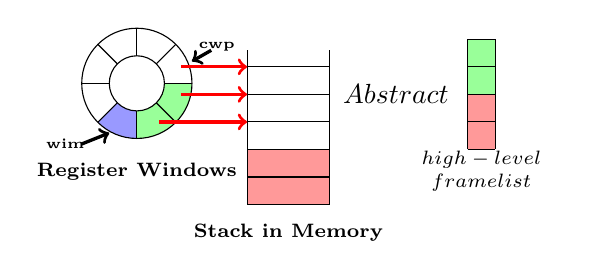
\begin{tikzpicture}[scale=0.7]
    \fill[green!40!white] (0,0) -- (0,-1cm) arc (-90:0:1cm) -- (0,0);
    \fill[blue!40!white] (0,0) -- (0,-1cm) arc (-90:-135:1cm) -- (0,0);
    % \fill[yellow!80!white] (0,0) -- (0,-1cm) arc (-90:-135:1cm) -- (0,0);
    % \fill[blue!40!white] (0,0) -- (-1,0cm) arc (-180:-135:1cm) -- (0,0);
    \draw (0, 0) -- (90:1cm);
    \draw (0, 0) -- (45:1cm);
    \draw (0, 0) -- (0:1cm);
    \draw (0, 0) -- (-45:1cm);
    \draw (0, 0) -- (-90:1cm);
    \draw (0, 0) -- (-135:1cm);
    \draw (0, 0) -- (-180:1cm);
    \draw (0, 0) -- (135:1cm);
    \fill[white] (0, 0) circle (0.5cm);
    \draw (0, 0) circle (1cm);
    \draw (0, 0) circle (0.5cm);
    % \draw[very thick, blue] (0, -0.3) -- (0, -1.2);
    % \draw[very thick, blue] (0, -0.32) -- (0.1, -0.32);
    % \draw[very thick, blue] (0, -1.18) -- (0.1, -1.18);
    \node(wim) at (-1.3, -1.1) {\tiny \bf wim};
    \draw[->, very thick] (-1, -1.1) -- (-0.5, -0.9);

    % \node(wim) at (-1.7, -0.7) {\tiny \bf wim};
    % \draw[->, very thick] (-1.5, -0.6) -- (-1, -0.4);
    

    \node(cwp) at (1.45, 0.67) {\tiny \bf cwp};
    \draw[->, very thick] (1.35, 0.6) -- (1, 0.4);

    \node(regwin) at (0, -1.6) {\scriptsize \bf Register Windows};

    %%%%%%%%%%%%%%%%%%%%%%%%%%%%%%%%%%%%%%%%%%%%%%%%%%%%%%

    \fill[red!40!white] (2, -1.2) rectangle (3.5, -1.7);
    \fill[red!40!white] (2, -1.7) rectangle (3.5, -2.2);

    \draw[-] (2, 0.6) -- (2, -2.2);
    \draw[-] (3.5, 0.6) -- (3.5, -2.2);
    
    \draw[-] (2, 0.3) -- (3.5, 0.3);
    \draw[-] (2, -0.2) -- (3.5, -0.2);
    \draw[-] (2, -0.7) -- (3.5, -0.7);
    \draw[-] (2, -1.2) -- (3.5, -1.2);
    \draw[-] (2, -1.7) -- (3.5, -1.7);
    \draw[-] (2, -2.2) -- (3.5, -2.2);

    \node(stkfm) at (2.75, -2.7) {\scriptsize \bf Stack in Memory};

    %%%%%%%%%%%%%%%%%%%%%%%%%%%%%%%%%%%%%%%%%%%%%%%%%%%%%%%

    \draw[->, very thick, red] (0.8, 0.3) -- (2, 0.3);
    \draw[->, very thick, red] (0.8, -0.2) -- (2, -0.2);
    \draw[->, very thick, red] (0.4, -0.7) -- (2, -0.7);

    %%%%%%%%%%%%%%%%%%%%%%%%%%%%%%%%%%%%%%%%%%%%%%%%%%%%%%

    \node(abstract) at (4.7, -0.2) {$\xLongrightarrow{\text{Abstract}}$};

    %%%%%%%%%%%%%%%%%%%%%%%%%%%%%%%%%%%%%%%%%%%%%%%%%%%%%%

    \fill[green!40!white] (6, 0.8) rectangle (6.5, 0.3);
    \fill[green!40!white] (6, 0.3) rectangle (6.5, -0.2);
    \fill[red!40!white] (6, -0.2) rectangle (6.5, -0.7);
    \fill[red!40!white] (6, -0.7) rectangle (6.5, -1.2);

    \draw[-] (6, 0.8) -- (6, -1.2);
    \draw[-] (6.5, 0.8) -- (6.5, -1.2);

    \draw[-] (6, 0.8) -- (6.5, 0.8);
    \draw[-] (6, 0.3) -- (6.5, 0.3);
    \draw[-] (6, -0.2) -- (6.5, -0.2);
    \draw[-] (6, -0.7) -- (6.5, -0.7);
    \draw[-] (6, -1.2) -- (6.5, -1.2);

    \node(hfrmlist) at (6.25, -1.6) 
        {
            \scriptsize \bf
            $
            \begin{array}{c}
                \text{high-level} \\
                \text{framelist}
            \end{array}
            $
        };
\end{tikzpicture} 
    \vspace*{-0.5em}
    \figurecaption{Abstraction of context management}
    \label{fig:Abstraction of Register Windows and Memory}
    \vspace{-0.5em}
\end{center}
During the execution of SPARCv8 program,
part of previous procedures' contexts
(the light gray part in the left side of
\Fig{\ref{fig:Abstraction of Register Windows and Memory}})
are saved in register window, the others
(the dark gray part in the left side of
\Fig{\ref{fig:Abstraction of Register Windows and Memory}})
are stored in stack in memory,
% (shown as the red arrow in
% \Fig{\ref{fig:Abstraction of Register Windows and Memory}}),
because the number of windows is limited.
The restriction is that the stack pointer
(\spreg{}) of each procedure,
including the current and previous ones,
whose context is saved in register
window currently, should point to the top of its stack frame
(shown as the thick arrow in
\Fig{\ref{fig:Abstraction of Register Windows and Memory}}),
so that the contexts
in these windows can be stored correctly
in memory when needed. For instance,
the context switch routine will check
whether the previous window is valid
(in clockwise direction in
\Fig{\ref{fig:Abstraction of Register Windows and Memory}}),
and use $\crestore{}$ instruction to set it as the
current one and save its contents into stack
(in memory) until the previous one
(filled with east north lines
in \Fig{\ref{fig:Abstraction of Register Windows and Memory}}) is invalid.
We require that the execution of client code
preserves such restriction. Otherwise, some SPARCv8
functions like context switch routine, whose
executions will store the contexts saved in
register windows into stack in memory, cannot be
verified if it is unclear where to save the
contents of some windows.
% We require the execution of client code
% preserving this relation so that the relation
% holds when calling context switch routine.
% \footnote{The requirement for client code
% preserving such relation will not restrict the
% application of our work, because such relation
% is also mentioned as a SPARCv8 programming
% convention in The SPARC Architecture Manual(version 8)~\cite{sparc},
% which says that "It is essential
% that \spreg{} always contains the correct value,
% so that when (and if) a register window overflow/underflow trap occurs,
% the register window can be correctly stored to or reloaded from memory "}.
% Otherwise, the correctness of context switch
% routine can't be proved if we are unclear where
% to save the contents of some windows.
We do the following when defining
Pseudo-SPARCv8 program to make the execution
of client code preserve such restriction:

\begin{itemize}
    \item
    In order to ensure that
    the stack pointer (\spreg{}) always
    points to the top of its stack frame, we require that
    each instruction, like \cadd{} and \ld{}, whose
    execution doesn't operate register window,
    is prohibited to update the value of \spreg{};
    and as for the \csave{} and \crestore{},
    % whose executions
    % will rotate register window,
    we require them
    to be used in specific forms.
    We introduce ``$\Psave \ \word$" as a macro of
    ``$\csave{} \ \spreg, -\word, \spreg$", whose execution
    generates a new \spreg{} pointing to the stack frame
    size $w$ allocated newly for the next window.
    We also introduce ``$\Prestore$"
    as a macro of ``$\crestore{} \ \greg{0}, \greg{0}, \greg{0}$"
    \footnote{In SPARCv8, $\greg{0}$ is always 0,
    and usually used as a parameter when instructions do not
    require a specific parameter.},
    whose execution just restores the previous window
    and doesn't modify the value of any register
    in the previous window restored.
    The original \csave{} and \crestore{} instructions
    have \textit{no} semantics in high-level client code.

    \item
    % The special registers can't be modified arbitrarily.
    The special registers in SPARCv8 usually play specific
    roles and modifying them should be done carefully.
    For example, \regwim{} marks which window is invalid.
    \begin{center}
        \vspace*{-0.5em}
        \begin{tikzpicture}[scale=0.75]
    \pgfdeclarepatternformonly{my crosshatch dots}{\pgfqpoint{-1pt}{-1pt}}{\pgfqpoint{2.5pt}{2.5pt}}{\pgfqpoint{3pt}{3pt}}
    {
        \pgfpathcircle{\pgfqpoint{0pt}{0pt}}{.4pt}
        \pgfpathcircle{\pgfqpoint{1.5pt}{1.5pt}}{.4pt}
        \pgfusepath{fill}
    }

    \fill[gray!20] (0,0) -- (0,-1cm) arc (-90:0:1cm) -- (0,0);
    \fill[pattern=my crosshatch dots] (0,0) -- (0,-1cm) arc (-90:-135:1cm) -- (0,0);
    \fill[pattern=north east lines] (0,0) -- (-1,0cm) arc (-180:-135:1cm) -- (0,0);
    \draw (0, 0) -- (90:1cm);
    \draw (0, 0) -- (45:1cm);
    \draw (0, 0) -- (0:1cm);
    \draw (0, 0) -- (-45:1cm);
    \draw (0, 0) -- (-90:1cm);
    \draw (0, 0) -- (-135:1cm);
    \draw (0, 0) -- (-180:1cm);
    \draw (0, 0) -- (135:1cm);
    \fill[white] (0, 0) circle (0.5cm);
    \draw (0, 0) circle (1cm);
    \draw (0, 0) circle (0.5cm);

    \node(wim) at (-1.7, -0.7) {\tiny \bf wim};
    \draw[->, line width=0.5pt] (-1.5, -0.6) -- (-1, -0.4);
    

    \node(cwp) at (1.45, 0.67) {\tiny \bf cwp};
    \draw[->, line width=0.5pt] (1.35, 0.6) -- (1, 0.4);

    \node(regwin) at (0, -1.6) {\scriptsize Register Windows};

    %%%%%%%%%%%%%%%%%%%%%%%%%%%%%%%%%%%%%%%%%%%%%%%%%%%%%%

    \fill[black!50] (2, -1.2) rectangle (3.3, -1.7);
    \fill[black!50] (2, -1.7) rectangle (3.3, -2.2);

    \draw[-] (2, 0.6) -- (2, -2.2);
    \draw[-] (3.3, 0.6) -- (3.3, -2.2);
    
    \draw[-] (2, 0.3) -- (3.3, 0.3);
    \draw[-] (2, -0.2) -- (3.3, -0.2);
    \draw[-] (2, -0.7) -- (3.3, -0.7);
    \draw[-] (2, -1.2) -- (3.3, -1.2);
    \draw[-] (2, -1.7) -- (3.3, -1.7);
    \draw[-] (2, -2.2) -- (3.3, -2.2);

    \node(stkfm) at (2.75, -2.7) {\scriptsize Stack in Memory};

    %%%%%%%%%%%%%%%%%%%%%%%%%%%%%%%%%%%%%%%%%%%%%%%%%%%%%%%

    \draw[->, line width=0.8pt] (0.8, 0.3) -- (2, 0.3);
    \draw[->, line width=0.8pt] (0.8, -0.2) -- (2, -0.2);
    \draw[->, line width=0.8pt] (0.4, -0.7) -- (2, -0.7);

    %%%%%%%%%%%%%%%%%%%%%%%%%%%%%%%%%%%%%%%%%%%%%%%%%%%%%%

    % \node(abstract) at (4.7, -0.2) {$\xLongrightarrow{\text{Abstract}}$};

    %%%%%%%%%%%%%%%%%%%%%%%%%%%%%%%%%%%%%%%%%%%%%%%%%%%%%%
\end{tikzpicture} 
        \figurecaption{Problem of modifying
        \regwim{} arbitrary}
        \vspace*{-0.5em}
        \label{fig:problem of modifying wim arbitrary}
    \end{center}
    If we change its value shown in
    \Fig{\ref{fig:Abstraction of Register Windows and Memory}}
    to mark another window invalid, as shown in
    \Fig{\ref{fig:problem of modifying wim arbitrary}},
    and call context switch routine to
    save the contents of previous windows into memory
    until the invalid one at this moment,
    a problem will arise since we don't know
    where to save the contents of window marked
    invalid originally
    (filled with dots
    in \Fig{\ref{fig:problem of modifying wim arbitrary}}).
    % Supposing the register window and
    So, we forbid the client
    to modify special registers and give \textit{no}
    semantics to instruction \cwr{} in high-level
    client code. Modifying them is hidden in the
    implementations of the abstract assembly primitives
    in low-level.
    And the delay buffer can be omitted in high-level
    program state.
    % omit them
    % in the Pseudo-SPARCv8 program state. Operating them
    % is hidden in the implementation of the
    % abstract assembly primitives.
    % We also do \textit{not} give semantics to
    % \cwr{} and \rd{} instructions in high-level
    % client code.
    \item
    As shown in \Fig{\ref{fig:Abstraction of Register Windows and Memory}},
    we find that we can abstract the register window
    and memory in stack storing contexts
    into a list (defined as
    HFrmList formally in \Fig{\ref{fig:machine-state-concur-pseudo-sparc}}).
    After this abstraction, we don't need to care about
    whether the contexts are saved in register windows or
    memory, and don't need to describe the contents of windows unused
    (the windows in white color in
    \Fig{\ref{fig:Abstraction of Register Windows and Memory}},
    but excluding the current one pointed by \regcwp{})
    in the Pseudo-SPARCv8 level.
    The \regcwp{} register is no longer needed in
    Pseudo-SPARCv8 program since the register windows
    are abstracted away.
    The low-level program in our work doesn't use this
    abstraction, because the low-level program
    should be realistically modelled,
    and the implementations of some primitives
    need to know the existance of register windows,
    for instance, the context switch routine
    needs to save the contents
    of the register window into stack (in memory).
\end{itemize}

\begin{figure*}[!t]
    \centering
    \small
    \[
        \begin{array}{rcclcrccl}
            \TYPE{(HCode)} & \ \HMd \ & \define & (\code, \hprimset) & &
            \qquad\,
            \TYPE{(CodeHeap)} & \ \code \ & \in & \TYPE{Word} \rightharpoonup \TYPE{Comm}
            \\
            \\[-8pt]
            \TYPE{(PrimSet)} & \hprimset & \define &
            \multicolumn{6}{l}
                {
                    \{ \lab{1} \rightsquigarrow \hprim_1, \dots, \lab{n} \rightsquigarrow \hprim_n \}
                    \qquad\quad
                    \TYPE{(Prim)} \ \ \hprim \ \in \
                    \TYPE{List} \ \TYPE{Val} \rightarrow \TYPE{HState} \rightarrow
                    \TYPE{HState} \rightarrow \TYPE{Prop}
                }  \\
            \\
            % \TYPE{(Prim)} & \hprim & \in &
            % \multicolumn{6}{l}
            % {
            %     \TYPE{List} \ \TYPE{Val} \rightarrow \TYPE{HState} \rightarrow
            %     \TYPE{HState} \rightarrow \TYPE{Prop}
            % } \\
            % \TYPE{(OpExp)} & \oexp & \define & \reg{} \sepline \val & &
            % \TYPE{(AddrExp)} & \aexp & \define & \oexp \sepline \reg{} + \oexp \\
            \TYPE{(Comm)} & \comm & \define &
            \multicolumn{6}{l}
            {
                \simplins{} \sepline \call{} \ \lab{}
                \sepline \jmp{} \ \aexp \sepline \retl \sepline \be{} \ \lab{}
            }
            \\
            \\[-8pt]
            \TYPE{(SimpIns)} & \simplins{} & \define &
            \multicolumn{6}{l}
            {
                % \csave{} \ \reg{s} \ \oexp \ \reg{d} \sepline
                % \crestore{} \ \reg{s} \ \oexp \ \reg{d} \sepline
                \Psave \ \word \sepline \Prestore  \sepline \cprint \ \reg{} \sepline
                \ld{} \ \aexp \ \reg{d} \sepline
                \st{} \ \reg{s} \ \aexp \sepline \cadd{} \ \reg{s} \ \oexp \ \reg{d}
                \sepline
                \rd \ \sr \ \reg{d} \sepline \cwr \ \reg{s} \ \oexp \ \sr
                % \sepline \dots
            }
            \\
            & & \quad | &
            \multicolumn{6}{l}
            {
                \csave{} \ \reg{s} \ \oexp \ \reg{d} \sepline
                \crestore{} \ \reg{s} \ \oexp \ \reg{d} \sepline
                \dots
            }
            \\
            \\[-8pt]
            \TYPE{(HMsg)} & \hmsg & \define & \empmsg \sepline \outEvt{\val} \sepline
            \callEvt{\lab{}, \args{\val}}
        \end{array}
    \]
    \vspace{-1em}
    \caption{Syntax of Pseudo-SPARCv8 Code}
    \label{fig:syntax-of-concur-pseudo-sparc}
\end{figure*}
\begin{figure*}[!t]
    \centering
    \small
    \vspace{-1em}
    \[
        \begin{array}{rcclrcclrccl}
            \TYPE{(HProg)} & \ \HProg \ & \define &
            (\HMd, \hpstate) &
            \qquad
            \TYPE{(HState)} & \ \hpstate \ & \define &
            (\thrdpool, \thrdid, \hthrdlocalst, \Mem) &
            \qquad
            \TYPE{(ThrdPool)} & \thrdpool & \define &
            \{ \thrdid \rightsquigarrow \hthrdlocalst \}^{*}
            \\
            \\[-8pt]
            \TYPE{(Tid)} & \thrdid & \in & \Ztype &
            \TYPE{(ThrdLcSt)} & \ \hthrdlocalst \ & \define &
            (\hRstate, \pc, \npc) &
            \TYPE{(HRstate)} & \hRstate & \define &
            (\hRfile, \hWstk) \\
            \\

            \TYPE{(HRegFile)} & \hRfile & \in &
            \multicolumn{9}{l}
            {
                \TYPE{HRegName} \rightarrow \TYPE{Val}
                \qquad\quad
                \TYPE{(HRegName)} \ \ \hrn \ \ \define \ \
                \reg{0} \sepline \dots \sepline \reg{31} \sepline
                \regn \sepline \regz \sepline \regc \sepline \regv
            }
            \\
            \\[-8pt]
            \TYPE{(HFrmList)} & \hWstk & \define &
            \multicolumn{9}{l}
            {
                \nil \sepline (\fm_1, \fm_2) \stCons \hWstk
                \qquad\qquad \ \
                \TYPE{(HFrame)} \ \ \fm \ \ \define \ \
                [\val_0, \dots, \val_7]
            }
        \end{array}
    \]
    % \vspace{-0.5em}
    \caption{Machine States for Pseudo-SPARCv8 Code}
    \label{fig:machine-state-concur-pseudo-sparc}
    % \vspace{-0.5em}
\end{figure*}

We define the syntax of the high-level Pseudo-SPARCv8 language
in \Fig{\ref{fig:syntax-of-concur-pseudo-sparc}}.
The code (\TYPE{HCode}) $\HMd$ has two parts:
the code heap $\code$
and the set of abstract primitives (\TYPE{PrimSet}) $\hprimset$,
which is a partial mapping from labels to
abstract assembly primitive. The code heap $\code$ in $\HMd$
acts as the client to
call abstract assembly primitives.
The abstract assembly primitive (\TYPE{Prim}) $\hprim$
is defined as a relation that takes a list of values
as arguments and maps a high-level program state
(defined in \Fig{\ref{fig:machine-state-concur-pseudo-sparc}})
to another.
% The definition of command and simple instruction are similar with
% the ones defined in \Fig{\ref{fig:Machine States and Language for SPARC Code}},
% except that we add two pseudo instructions $\Psave \ \word$ and $\Prestore$
% in simple instruction.
% Comparing the simple instruction with the one shown in
% \Fig{\ref{fig:Machine States and Language for SPARC Code}},
% we add three pseudo instructions.
We add three pseudo instructions in simple instruction (\TYPE{SimpIns}).
The $\Psave \ \word$
and $\Prestore$ restrict the instruction \csave{}
and \crestore{} to be used in the specific form as
mentioned before.
We also introduce $\cprint \ \reg{}$,
whose execution outputs the value $\val$ in
general register $\reg{}$ and
generates an message $\outEvt{\val}$
as an observable event.
% whose execution will occur an output $\outEvt{\val}$,
% to generate observable events.
The high-level message (\TYPE{HMsg})
$\hmsg$ can be either an empty message $\empmsg$, or an output
$\outEvt{\val}$, or a $\callEvt{\lab{}, \args{\val}}$ meaning to
call a primitive labelled $\lab{}$ with arguments $\args{\val}$.

The machine states \TYPE{(HState)}
of the high-level Pseudo-SPARCv8 program
are defined in \Fig{\ref{fig:machine-state-concur-pseudo-sparc}}.
The high-level program $\HProg$ is a pair of high-level code
$\HMd$ and high-level state $\hpstate$. High-level
state is a tuple including: 
a thread pool (\TYPE{ThrdPool}) $\thrdpool$,
% the identifier of the current thread $\thrdid$,
current thread id (\TYPE{Tid}) $\thrdid$, 
the thread local state (\TYPE{ThrdLcSt}) $\hthrdlocalst$ 
of the current thread, and the memory (\TYPE{Mem}) $\Mem$.

\begin{figure*}[!t]
    \centering
    \small
    \vspace*{-0.5em}
    \subfigure[High-level Program Transition]{
        \begin{minipage}[b]{1\textwidth}
        \[
            \begin{array}{c}
                \infer
                {
                    \HGlobTrans{(\HMd, (\thrdpool, \thrdid, \hthrdlocalst, \Mem))}
                    { \empmsg }{(\HMd, (\thrdpool, \thrdid, \hthrdlocalst', \Mem'))}
                }
                {
                    \HMd = (\code, \hprimset) \quad \ \
                    \hlocalstep{\code}{(\hthrdlocalst, \Mem)}{ \ \empmsg \ }
                        {(\hthrdlocalst', \Mem')}
                } \qquad \quad
                \infer
                {
                    \HGlobTrans{(\HMd, (\thrdpool, \thrdid, \hthrdlocalst, \Mem))}
                    { \outEvt{\val} }{(\HMd, (\thrdpool, \thrdid, \hthrdlocalst', \Mem))}
                }
                {
                    \HMd = (\code, \hprimset) \quad \ \
                    \hlocalstep{\code}{(\hthrdlocalst, \Mem)}{\outEvt{\val}}
                        {(\hthrdlocalst', \Mem)}
                } \\
                \\
                \infer
                {
                    \HGlobTrans{(\HMd, (\thrdpool, \thrdid, \hthrdlocalst, \Mem))}
                    {\empmsg}
                    {(\HMd, (\thrdpool', \thrdid', \hthrdlocalst'', \Mem'))}
                }
                {
                    \begin{array}{c}
                        \HMd = (\code, \hprimset) \quad \ \
                        \hlocalstep{\code}{(\hthrdlocalst, \Mem)}
                            {\callEvt{\lab{}, \args{\val}}}
                            {(\hthrdlocalst', \Mem)} \quad \ \
                        \hprimset(\lab{}) = \hprim \\
                        \hprim \, (\args{\val})(\thrdpool, \thrdid, \hthrdlocalst', \Mem)
                            (\thrdpool', \thrdid', \hthrdlocalst'', \Mem')
%                    	\quad \ \
%                    	\{\hthrdlocalst''.\pc, \hthrdlocalst''.\npc\}
%                    	\subseteq \dom(\code)
                    \end{array}
                }
            \end{array}
        \]
        \vspace{0.2em}
        \end{minipage}
    }

    \subfigure[High-level Thread Local Transition]
    {
        \begin{minipage}[b]{1\textwidth}
        \[
            \begin{array}{c}
                \infer
                {
                    \hlocalstep{\code}{((\hRstate, \pc, \npc), \Mem)}
                        { \ \empmsg \ }
                        {((\hRstate', \npc, \npc + 4), \Mem')}
                }
                {
                    \code(\pc) = \simplins{} \quad \ \
                    \hexeci{\simplins{}}{(\hRstate, \Mem)}{(\hRstate', \Mem')}
                } \\
                \\
                \infer
                {
                    \hlocalstep{\code}{(((\hRfile, \hWstk), \pc, \npc), \Mem)}
                        { \ \empmsg \ }
                        {(((\hRfile\{ \reg{15} \rightsquigarrow \pc \},
                            \hWstk), \npc, \lab{}), \Mem)}
                }
                {
                    \code(\pc) = \call{} \ \lab{} \quad \reg{15} \in \dom(\hRfile)
                } \\
                \\
                \infer
                {
                    \hlocalstep{\code}{(((\hRfile, \hWstk), \pc, \npc), \Mem)}
                        { \ \empmsg \ }
                        {(((\hRfile, \hWstk), \npc, \lab{}+8), \Mem)}
                }
                {
                    \code(\pc) = \retl{} \quad \ \ \hRfile(\reg{15}) = \lab{}
                } \\
                \\
                \infer
                {
                    \hlocalstep{\code}{(((\hRfile, \hWstk), \pc, \npc), \Mem)}
                        { \outEvt{\val} }
                        {(((\hRfile, \hWstk), \npc, \npc+4), \Mem)}
                }
                {
                    \code(\pc) = \cprint \ \reg{} \quad \ \ \hRfile(\reg{}) = \val
                } \\
                \\
                \infer
                {
                    \hlocalstep{\code}
                    {((\hRstate, \pc, \npc), \Mem)}
                        { \callEvt{\pc, \args{\val}} }
                        {((\hRstate, \pc, \npc), \Mem)}
                }
                {
                    \pc \notin \dom(\code) \quad \ \
                    \npc = \pc\!+\!4 \quad \ \
                    \arguments(\hRstate, \Mem, \args{\val})
                }
            \end{array}
        \]
        \vspace{0.2em}
        \end{minipage}
    }

    \subfigure[High-level Instruction Transition]
    {
        \begin{minipage}[b]{1\textwidth}
        \[
            \begin{array}{c}
                \infer
                {
                    \hexeci{\Psave \ \word}{(\hRstate, \Mem)}{(\hRstate', \Mem')}
                }
                {
                    \begin{array}{c}
                        \hRstate =  (\hRfile, \hWstk) \quad \ \
                        \hRfile' = \hRfile\{ \outRN  \rightsquigarrow \notCare,
                            \localRN \rightsquigarrow \notCare,
                            \inRN \rightsquigarrow \hRfile([\outRN]) \}
                        \{ \spreg \rightsquigarrow (\block, 0) \} \\
%                        \hRfile(\spreg) = (\block_0, 0) \quad \ \
                        \malloc(\Mem, \block, 64, \word) = \Mem' \quad \ \
                        \hRstate' =
                        (\hRfile', (\hRfile([\localRN]),
                            \hRfile([\inRN])) \stCons \hWstk)
                    \end{array}
                } \\
                \\
                \infer
                {
                    \hexeci{\Prestore}{(\hRstate, \Mem)}{(\hRstate', \Mem')}
                }
                {
                    \begin{array}{c}
                        \hRstate = (\hRfile, (\fm_1, \fm_2)
                            \stCons \hWstk) \quad \ \
                        \hRfile(\spreg) = (\block, 0) \quad \ \
                        \mfree(\block, \Mem) = \Mem'
%                        \quad \ \
%                        \hRfile'(\spreg) = (\block_0, 0)
                        \\
                        \hRfile' = \hRfile\{ \outRN \rightsquigarrow
                            \hRfile([\inRN]), \localRN \rightsquigarrow \fm_1,
                            \inRN \rightsquigarrow \fm_2 \} \quad \ \
                        \hRstate' = (\hRfile', \hWstk)
                    \end{array}
                }
            \end{array}
        \]
        \vspace{0.2em}
        \end{minipage}
    }
    \caption{Selected operational semantics rules for high-level program}
    \label{fig:selected-opsem-high-level-prog}
\end{figure*}

\paragraph{\textbf{Thread Local State.}}
The thread local state $\hthrdlocalst$
is a triple of high-level register state
\TYPE{(HRstate)} $\hRstate$,
and program counters $\pc$ and $\npc$. The high-level
register state $\hRstate$ consists of
the high-level register file (\TYPE{HRegFile}) $\hRfile$,
% the block of the current stack frame $\block$,
and the high-level frame list (\TYPE{HFrmList}) $\hWstk$.
$\hrn$ is the high-level register names (\TYPE{HRegName}), 
where the $\regcwp$ register is omitted as introduced before and
we also omit special registers for simplicity,
because we forbid
the high-level client code to modify them
\footnote{There is no problem to reserve special
registers in high-level register file and permit
the high-level client code to read them.}.
The high-level frame list $\hWstk$ is a list of pairs
$(\fm_1, \fm_2)$, which is used to save
% the block id $\block$ of the stack frame and
the contexts (\localRN{} and \inRN{} registers)
$\fm_1$ and $\fm_2$ of previous procedures.
After introducing the state of high-level program,
we define the primitive $\primsw$ as
an instantiation of $\hprim$ below:
\[
    \small\!\!
    \begin{array}{l}
        \primsw \ \define \\
        \quad
        \lambda \, \args{\val}, \hpstate, \hpstate'. \
        \exists \, \thrdid'. \
        \Mem(\TaskNew) = (\thrdid', 0) \land
        \thrdpool(\thrdid') =
            (\hRstate', \pc', \npc') \\
        \qquad\qquad
        \land \,
        \thrdpool' = \thrdpool\{ \thrdid \rightsquigarrow
            (\hRstate, \pc, \npc) \}
            \land \tid \neq \tid' \land \args{\val} = \nil \\
        \\[-9pt]
        \quad \text{where} \
        \hpstate =
            (\thrdpool, \thrdid, (\hRstate, \pc, \npc), \Mem), \\
        % \tid \in \dom(\thrdpool)
        \qquad\qquad
        \hpstate' =
            (\thrdpool', \thrdid',
                (\hRstate', \lab{}\!+\!8, \lab{}\!+\!12), \Mem),
                \lab{} = \hRstate'.\hRfile(\reg{15}).
    \end{array}
\]
% {
%     \small
%     $$
%     \begin{array}{lcl}
%         \primsw & \define &
%         \lambda \, \args{\val}, \hpstate, \hpstate'. \
%         \exists \, \thrdid'. \
%         \Mem(\TaskNew) = (\thrdid', 0) \, \land \,
%         \thrdpool(\thrdid') =
%             (\hRstate', \pc', \npc') \\
%         & & \hspace*{8em} \land \,
%         \thrdpool' = \thrdpool\{ \thrdid \rightsquigarrow
%         (\hRstate, \pc, \npc) \}
%         \, \land \, \thrdid \neq \thrdid'
%         \, \land \, \args{\val} = \nil \\
%         \\[-8pt]
%         \multicolumn{3}{l}
%         {
%         	\hspace*{1.8em}
%             \TYPE{where } \,
%             \hpstate =
%                 (\thrdpool, \thrdid, (\hRstate, \pc, \npc), \Mem), \,
%             \hpstate' =
%             (\thrdpool', \thrdid',
%             	(\hRstate', \lab{} + 8, \lab{} + 12), \Mem), \lab{} = \hRstate'.\hRfile(\reg{15}).
% %            \lab{} = \hRstate'.\hRfile(\reg{15}).
%             % \,
%             % \AftExt(\hRstate, \pc, \npc) \define
%             % (\hRstate, \hRstate.\hRfile(\reg{15}) + 8,
%             %     \hRstate.\hRfile(\reg{15}) + 12)
%         }
%     \end{array}
%     $$
% }
The $\primsw{}$ primitive takes no arguments
($\args{\val} = \nil$), and changes the identifier
of the current thread according to the value
in the location $\TaskNew$. We use parameters $\hpstate$
and $\hpstate'$ to represent the machine states before
and after execution of $\primsw{}$ respectively.

\paragraph{\textbf{Operational Semantics in High-level.}}
The operational semantics for high-level Pseudo-SPARCv8 program
is defined in \Fig{\ref{fig:selected-opsem-high-level-prog}}.
The high-level program transition relation
$\HGlobTrans{(\HMd, \hpstate)}{\hmsg}{(\HMd, \hpstate')}$ is defined
in \Fig{\ref{fig:selected-opsem-high-level-prog}} (a). In each step,
the program may either execute the instruction pointed by $\pc$
and generate empty message $\empmsg$ or an output $\outEvt{\val}$,
or call  an abstract assembly primitive in the primitive set.
When calling an abstract assembly primitive,
the execution of current thread (defined as
$(\hlocalstep{\notCare}{\notCare}{\ \notCare \ }{\notCare})$ in
\Fig{\ref{fig:selected-opsem-high-level-prog}} (b)) will generate
a message $\callEvt{\lab{}, \args{\val}}$, which means that it
hopes to call the abstract assembly primitive $\hprim$ labelled
$\lab{}$, which is {\it not} in the domain of code heap $\code$,
with the arguments $\args{\val}$
(we use $\arguments(\hRstate, \Mem, \args{\val})$
to get the arguments $\args{\val}$
from high-level state, and its definition is omitted here).
%After executing the abstract assembly primitive, the program
%control transfer should return to execute the client code
%(shown as $\{\hthrdlocalst''.\pc, \hthrdlocalst''.\npc\}
%\subseteq \dom(\code)$).

The thread local step is defined in
\Fig{\ref{fig:selected-opsem-high-level-prog}} (b)
Here, the step for simple instruction $\simplins{}$ is
represented as ``$\hexeci{\simplins{}}{\notCare}{\notCare}$".
We show the state transition relation for pseudo instructions
$\Psave \ \word$ and $\Prestore$ in
\Fig{\ref{fig:selected-opsem-high-level-prog}} (c).
Supposing the current register state $\hRstate$ is
$(\hRfile, \hWstk)$, the execution of
$\Psave \ \word$ will save the \localRN{} and \inRN{} registers
% and the block id  $\block_0$ of the current stack frame
into high-level frame list $\hWstk$. It also allocates
a new block $\block$ of size 64 byte to $\word$ byte
as a new stack frame in memory
(represented as $\malloc(\Mem, \block, 64, \word) = \Mem'$).
% The size of the block $\block$ is from 64 byte to $\word$ byte.
The reason why it starts from 64 byte is that the 0 to 64 bytes
(16 words) in a stack frame are usually reserved to save
the context in window (\localRN{} and \inRN{} registers)
by convention \cite{sparc},
and this part of memory is abstracted away in
Pseudo-SPARCv8 program as we have explained and shown in
\Fig{\ref{fig:Abstraction of Register Windows and Memory}}.
$\Prestore$ does the reverse,
freeing the block of the current stack frame
(represented as $\mfree(\block, \Mem) = \Mem'$), and
restoring the context of the previous procedure
saved in $\hWstk$.
% More details of the high-level Pseudo
% SPARCv8 program can be seen in Appendix \ref{appendix:more-about-high-level-insExec}.

\subsection{Low-level SPARCv8 Program}
\label{subsec:low-level SPARCv8 Program}

% The low-level \sparc{} program are very closed to the \sparc{} program
% defined in \Fig{\ref{fig:Machine States and Language for SPARC Code}}.
% The only difference here is that we use simple instructions and commands
% defined in \Fig{\ref{fig:syntax-of-concur-pseudo-sparc}}. So, the global
% program transition of the low-level \sparc{} program is defined as
% the following form :

The global program transition of the low-level \sparc{} program is defined
as the following form:
\[
    \scriptsize
    \infer
    {
        \LGlobTrans{(\code, (\Mem, (\RFile, \Wstack), \DBuf), \pc, \npc)}
            { \empmsg / \outEvt{\val} }
            {(\code, (\Mem', (\RFile'', \Wstack'), \DBuf''), \pc', \npc')}
    }
    {
        \begin{array}{l}
            \Dstep{(\RFile, \DBuf)}{(\RFile', \DBuf')} \\
            \llocalstep{\code}
                {((\Mem, (\RFile', \Wstack), \DBuf'), \pc, \npc)}
                { \empmsg / \outEvt{\val} }
                {((\Mem', (\RFile'', \Wstack'), \DBuf''), \pc', \npc')}
        \end{array}
    }
\]
The low-level \sparc{} program is slightly different
from the \sparc{} program defined in
\Sec{\ref{sec:modeling}}:
\begin{enumerate}
    \item The low-level \sparc{} program uses the
        instructions defined in
        \Fig{\ref{fig:syntax-of-concur-pseudo-sparc}}.
        It means that we need to give semantics to the %additional
        pseudo instructions $\Psave$, $\Prestore$ and
        $\cprint$ in the low-level \sparc{} program.
        Since $\Psave$ and $\Prestore$
        are simply special forms of $\csave{}$ and
        $\crestore{}$ as explained,
        and $\cprint$ is a primitive
        responsible for generating observable events,
        %which does the same thing as the high-level one,
        defining their semantics is not a challenge
        and the translation of programs in this modified language 
        into ones in the standard \sparc{} language is 
        trivial.
    \item The program transition defined in
        \Sec{\ref{sec:modeling}} does not generate
        observable events. 
        Here, Since we want to support refinement verification 
        and use the event trace refinement~\cite{liang14lics}, 
        % Here, in order to support
        % refinement verification, since
        % we use the event trace refinement~\cite{liang14lics},
        each step of the program
        generates either an empty message $\tau$,
        or an output $\outEvt{\val}$ produced
        by $\cprint$.
\end{enumerate}

% Each step of the program produces either an empty message $\empmsg$, or
% an output $\outEvt{\val}$ that is produced by the instruction
% $\cprint$ and acts as an observable behavior.
Note that the client
code and the implementations of abstract assembly primitives
in the low-level are both \sparc{} code heap. So, we do not need
to define their linking in semantics.
More details of the low-level program can be found in
our Coq code and TR~\cite{coqimp}.
% \ref{sec:more-llang}.

% \begin{figure*}[!htb]
    \centering
    \begin{tikzpicture}[scale=1.2, font=\scriptsize]
        \node(low-level) at (-0.8, 2) {\bf \scriptsize \color{blue} Low-level};
        \node(memT) at (3, 2) {$\Mem_T = \Mem_1 \uplus \dots \uplus \Mem_n$};
        \node(TaskCur) at (6.5, 2) {$\{ \TaskCur \rightsquigarrow (\thrdid, 0) \}$};
        \node(CurStateLow) at (9, 2) {$\Rstate, \, \Mem_c$};
        \node(sharedMem) at (10.5, 2) {$\Mem'$};

        %%%%%%%%%%%%%%%%%%%%%%%%%%%%%%%%%%%%%%%%%%%%%%%%%%%%%

        \draw[->] (2.7, 1.8) -- (2.42, 0.2);
        \draw[->] (3.9, 1.8) -- (3.9, 0.2);
        \draw[->] (6.5, 1.8) -- (6.5, 0.2);
        \draw[->] (9, 1.8) -- (9, 0.2);
        \draw[->] (10.5, 1.8) -- (10.5, 0.2);
        \draw[-,dashed, green] (-0.7, 1) -- (11, 1);

        %%%%%%%%%%%%%%%%%%%%%%%%%%%%%%%%%%%%%%%%%%%%%%%%%%%%%

        \node(high-level) at (-0.8, 0) {\bf \scriptsize \color{red} High-level};
        \node(T) at (2.8, 0) {$\thrdpool\backslash\{ \thrdid \} = 
            \{ \thrdid_1 \rightsquigarrow \hthrdlocalst_1, \dots, 
                \thrdid_n \rightsquigarrow \hthrdlocalst_n \}$};
        \node(Tid) at (6.5, 0) {$\thrdid$};
        \node(CurStateHigh) at (9, 0) {$\hthrdlocalst$};
        \node(sharedMem) at (10.5, 0) {$\Mem'$};
    \end{tikzpicture} 
    \caption{State Relation between Low- and High-level Program State}
    \label{fig:State Relation between Low- and High-level Program State}
\end{figure*}
\subsection{Primitive Correctness}
\label{subsec:correctness-primitive}

We first establish a state relation
between low- and high-level program states.
We define this relation below 
($\uplus$ means disjoint union), shown as
``$\stateRel{\state}{\hpstate}$".
\[
    \small
    \infer
    {
        \stateRel{(\Mem, \Rstate, \DBuf)}
            {(\thrdpool, \thrdid, \hthrdlocalst, \Mem')}
    }
    {
        \begin{array}{c}
            \Mem = \Mem_c \uplus \Mem_T \uplus
                \{ \TaskCur \rightsquigarrow (\thrdid, 0) \}
                \uplus \Mem' \\
            \curStRel{(\Mem_c, \Rstate)}{(\thrdid, \hthrdlocalst)}
            \quad \ \
            \rdyStRel{\Mem_T}{\thrdpool \backslash \{ \thrdid \}}
            \quad \ \
            \DBuf = \nil
        \end{array}
    }
\]
The low-level memory $\Mem$ is split into four parts:
$\Mem_c$ used to save the context of the current thread $\thrdid$;
$\Mem_T$ saving the contexts of the ready threads,
except the current thread $\tid$; a singleton memory
cell located $\TaskCur$ saving the current thread id; and shared
memory $\Mem'$ that is same as the high-level memory.
The delayed buffer $\DBuf$ is $\nil$, because client
is not permitted to modify any special register
through the $\cwr{}$ instructions. The memory $\Mem_T$ used to
save the contexts of the ready threads is {\it abstracted} as a thread pool
in high-level program. Their relation is represented as
``$\rdyStRel{\Mem_T}{\thrdpool \backslash \{ \thrdid \}}$".
We use ``$\curStRel{(\Mem_c, \Rstate)}{(\thrdid, \hthrdlocalst)}$"
to represent the state relation of the current thread
in low- and high-level programs.
% Full definitions of the state relation
% can be found in Appendix \ref{sec:more-staterel}.

The correctness of abstract assembly primitives
is defined in terms of {\it contextual refinement}.
We give its formal definition in
\Def{\ref{def:prim-correctness}}.
And we use the {\it event trace refinement}
proposed by \etal{Liang} \cite{liang14lics}.

\begin{definition}[Primitive Correctness]
    \label{def:prim-correctness}
    {\em $\asmimp \ctxrefine \hprimset$} iff  \\
    for any {\em $\code$}, {\em $\state$}, {\em $\hpstate$}, 
    {\em $\pc$} and {\em $\npc$}, if
    {\em $\stateRel{\state}{\hpstate}$}, and {\em $\progsafe(\HProg)$},
    then {\em $\prog \refine \HProg$} holds.
    (where {\em $\prog = (\code \uplus \asmimp, \state, \pc, \npc)$}, \,
        {\em $\HProg = ((\code, \hprimset), \hpstate)$}, and
        {\em $\hpstate.\hthrdlocalst = (\notCare, \pc, \npc)$}).
\end{definition}

We use a code heap $\asmimp$
% , which is a code heap,
to represent the implementations
 and $\hprimset$ to represent the set of corresponding
abstract assembly primitives.
The contextual refinement,
denoted as $\asmimp \ctxrefine \hprimset$,
says that if and only if for any client code
(or context) $\code$, low-level program
state $\state$, high-level program state $\hpstate$, program counters
$\pc$ and $\npc$, if the low- and high-level program states satisfy the
state relation $\stateRel{\state}{\hpstate}$ and the high-level program
will never get stuck (shown as $\progsafe(\HProg)$),
then there is an {\it event trace refinement}~\cite{liang14lics},
which means that $\prog$ produces no more observable behaviors
than $\HProg$ and is denoted as $\prog \refine \HProg$,
between low- and high-level programs. $\progsafe(\HProg)$
% which means that the high-level program will never get stuck,
is defined formally below:
\[
    \small
    \progsafe(\HProg) \ \define \
    \forall \, \HProg'. \,
    (\HGlobMultiTrans{\HProg}{}{*}{\HProg'})
    \Longrightarrow
    (\exists \, \HProg''. \,
        \HGlobTrans{\HProg'}{}{\HProg''})
\]
The client code $\code$ is \sparc{} code, so
the high-level code is a pair of $\code$ and $\hprimset$,
% And their linking is defined in
% \Fig{\ref{fig:selected-opsem-high-level-prog}}.
and the low-level code is just the union of
$\code$ and $\asmimp$, shown as
$(\code\uplus\asmimp)$, because both of
$\code$ and $\asmimp$ are \sparc{} code heap:
\[
    \small
    \code \uplus \asmimp \,\define\,
    \code \cup \asmimp \quad
    \cif \ \dom(\code)\cap\dom(\asmimp) = \emptyset
\]

% \subsection{State Relation between Low- and High-level Program}
% \label{subsec:state-rel}
% % According to previous research works about refinement verification,
% % \eg{\cite{CompCert,Liang12popl}}, one of the important thing to achieve
% % refinement verification is to establish the states relation between
% % low- and high-level program.
% In order to achieve refinement verification, we need to
% establish a relation as an {\it invariant}
% between low- and high-level program state.
% We define this relation below, shown as
% ``$\stateRel{\state}{\hpstate}$".
% % We illustrate this relation, defined as
% % ``$\stateRel{\state}{\hpstate}$"
% % formally below, with \Fig{\ref{fig:State Relation between
% % Low- and High-level Program State}}.
% \[
%     \small
%     \infer
%     {
%         \stateRel{(\Mem, \Rstate, \DBuf)}
%             {(\thrdpool, \thrdid, \hthrdlocalst, \Mem')}
%     }
%     {
%         \begin{array}{c}
%             \Mem = \Mem_c \uplus \Mem_T \uplus
%                 \{ \TaskCur \rightsquigarrow (\thrdid, 0) \}
%                 \uplus \Mem' \\
%             \curStRel{(\Mem_c, \Rstate)}{(\thrdid, \hthrdlocalst)}
%             \quad \ \
%             \rdyStRel{\Mem_T}{\thrdpool \backslash \{ \thrdid \}}
%             \quad \ \
%             \DBuf = \nil
%         \end{array}
%     }
% \]
% % \begin{figure}[!h]
% %     \centering
% %     \small
% %     \[
% %         \infer
% %         {
% %             \stateRel{(\Mem, \Rstate, \DBuf)}
% %                 {(\thrdpool, \thrdid, \hthrdlocalst, \Mem')}
% %         }
% %         {
% %             \begin{array}{c}
% %                 \Mem = \Mem_c \uplus \Mem_T \uplus
% %                     \{ \TaskCur \rightsquigarrow (\thrdid, 0) \}
% %                     \uplus \Mem' \\
% %                 \curStRel{(\Mem_c, \Rstate)}{(\thrdid, \hthrdlocalst)}
% %                 \quad \ \
% %                 \rdyStRel{\Mem_T}{\thrdpool \backslash \{ \thrdid \}}
% %                 \quad \ \
% %                 \DBuf = \nil
% %             \end{array}
% %         }
% %     \]
% %     \vspace{-1.5em}
% %     \caption{Relation for Whole Program State}
% %     \label{fig:rel-wp}
% %     \vspace{-0.5em}
% % \end{figure}

% The low-level memory $\Mem$ is splitted into four parts:
% $\Mem_c$ used to save the context of the current thread $\thrdid$;
% $\Mem_T$ saving the contexts of the ready threads,
% except the current thread $\tid$; a singleton memory
% cell located $\TaskCur$ saving the current thread id; and shared
% memory $\Mem'$.
% % Note, ready threads are threads in thread pool,
% % except the current thread $\thrdid$.
% The delayed buffer $\DBuf$ is $\nil$, because client
% code is not permitted to modify special register by
% $\cwr{}$ instruction.
% The memory $\Mem_T$ used to
% save the contexts of the ready threads is {\it abstracted} as a thread pool
% in high-level program. Their relation is represented as
% ``$\rdyStRel{\Mem_T}{\thrdpool \backslash \{ \thrdid \}}$".
% We use ``$\curStRel{(\Mem_c, \Rstate)}{(\thrdid, \hthrdlocalst)}$"
% to represent the state relation of current thread $\thrdid$
% in low- and high-level program.
% Full definitions of the state relation
% can be found in Appendix \ref{sec:more-staterel}.

% % \begin{figure*}[!t]
% %     \centering
% %     \[
% %         \begin{array}{c}
% %             \TYPE{(EvtTrace)} \ \ \evttr \ \define \
% %             \outEvt{\val} \stCons \evttr \sepline \nil \sepline
% %             \evtabort \quad \ \ \TYPE{(co-inductive)} \\
% %             \\
% %             \infer=
% %             {
% %                 \Etr{(\prog, \evtabort)}
% %             }
% %             {
% %                 \neg
% %                 (\exists \, \prog'. \
% %                  \LGlobMultiTrans{\prog}{}{+}{\prog'})
% %             } \qquad \ \
% %             \infer=
% %             {
% %                 \Etr{(\prog, \nil)}
% %             }
% %             {
% %                 \LGlobMultiTrans{\prog}{ \, \empmsg \ }{+}{\prog'}
% %                 \quad \ \
% %                 \Etr{(\prog', \nil)}
% %             } \quad \ \
% %             \infer=
% %             {
% %                 \Etr{(\prog, \outEvt{\val} \stCons \evttr)}
% %             }
% %             {
% %                 \LGlobMultiTrans{\prog}{\!\!\outEvt{\val}\!}{+}{\prog'}
% %                 \quad \ \
% %                 \Etr{(\prog', \evttr)}
% %             }
% %             % \\
% %             % \\[-5pt]
% %             % \infer=
% %             % {
% %             %     \Etr{(\HProg, \evtabort)}
% %             % }
% %             % {
% %             %     \neg
% %             %     (\exists \, \HProg'. \
% %             %      \HGlobMultiTrans{\HProg}{}{+}{\HProg'})
% %             % } \qquad \ \
% %             % \infer=
% %             % {
% %             %     \Etr{(\HProg, \nil)}
% %             % }
% %             % {
% %             %     \HGlobMultiTrans{\HProg}{ \, \empmsg \ }{+}{\HProg'}
% %             %     \quad \ \
% %             %     \Etr{(\HProg', \nil)}
% %             % } \quad \ \
% %             % \infer=
% %             % {
% %             %     \Etr{(\HProg, \outEvt{\val} \stCons \evttr)}
% %             % }
% %             % {
% %             %     \HGlobMultiTrans{\HProg}{\!\!\outEvt{\val}\!}{+}{\HProg'}
% %             %     \quad \ \
% %             %     \Etr{(\HProg', \evttr)}
% %             % } \\
% %             % \\
% %             % \prog \refine \HProg \ \define \
% %             %     \forall \, \evttr. \,
% %             %     \Etr{(\prog, \evttr)} \Longrightarrow
% %             %     \Etr{(\HProg, \evttr)}
% %         \end{array}
% %     \]
% %     \caption{Event Trace Refinement}
% %     \label{fig:event-trace-refinement}
% % \end{figure*}

% \subsection{Correctness of Abstract Assembly Primitive}
% \label{subsec:correctness-primitive}

% The correctness of abstract assembly primitive can be defined in terms of
% {\it contextual refinement}.
% Below we will give the formal definition in
% \Def{\ref{def:prim-correctness}}.
% And we use {\it event trace refinement}
% proposed by \etal{Liang} \cite{liang14lics}.

% \begin{definition}[Primitive Correctness]
%     \em
%     \label{def:prim-correctness}
%     $\asmimp \refine \hprimset$ iff  \\
%     for any $\code, \, \state, \, \hpstate, \, \pc$ and $\npc$, if
%     $\stateRel{\state}{\hpstate}$, and $\progsafe(\HProg)$,
%     then $\prog \refine \HProg$ holds.
%     % \\
%     % \\[-9pt]
%     (where $\prog = (\code \uplus \asmimp, \state, \pc, \npc), \,
%         \HProg = ((\code, \hprimset), \hpstate)$, and
%         $\hpstate.\hthrdlocalst = (\notCare, \pc, \npc)$).
% \end{definition}

% Here, we use a code heap $\asmimp$
% % , which is a code heap,
% to represent the implementations of abstract
% assembly primitives and $\hprimset$ to represent the set of corresponding
% abstract assembly primitives. The contextual refinement between
% $\asmimp$ and $\hprimset$, denoted as $\asmimp \refine \hprimset$,
% says that if and only if for any client code
% (or context) $\code$, low-level program
% state $\state$, high-level program state $\hpstate$, program counters
% $\pc$ and $\npc$, if the low- and high-level program states satisfy the
% state relation $\stateRel{\state}{\hpstate}$ and the high-level program
% will never get stuck (shown as $\progsafe(\HProg)$),
% then there is an {\it event trace refinement} relation
% between low- and high-level program. The property $\progsafe(\HProg)$,
% % which means that the high-level program will never get stuck,
% is defined below formally :
% \[
%     \progsafe(\HProg) \ \define \
%     \forall \, \HProg'. \,
%     (\HGlobMultiTrans{\HProg}{}{*}{\HProg'})
%     \Longrightarrow
%     (\exists \, \HProg''. \,
%         \HGlobTrans{\HProg'}{}{\HProg''})
% \]

% \paragraph{\textbf{Event Trace Refinement.}}
% We define the event trace refinement co-inductively
% in \Fig{\ref{fig:event-trace-refinement}}.
% \begin{center}
%     \[
%         \small
%         \begin{array}{c}
%             \TYPE{(EvtTrace)} \ \ \evttr \ \define \
%             \outEvt{\val} \stCons \evttr \sepline \nil \sepline
%             \evtabort \quad \ \ \TYPE{(co-inductive)} \\
%             \\
%             \infer=
%             {
%                 \Etr{(\prog, \evtabort)}
%             }
%             {
%                 \neg
%                 (\exists \, \prog'. \
%                  \LGlobMultiTrans{\prog}{}{+}{\prog'})
%             } \qquad \ \
%             \infer=
%             {
%                 \Etr{(\prog, \nil)}
%             }
%             {
%                 \LGlobMultiTrans{\prog}{ \, \empmsg \ }{+}{\prog'}
%                 \quad \ \
%                 \Etr{(\prog', \nil)}
%             } \\
%             \infer=
%             {
%                 \Etr{(\prog, \outEvt{\val} \stCons \evttr)}
%             }
%             {
%                 \LGlobMultiTrans{\prog}{\!\!\outEvt{\val}\!}{+}{\prog'}
%                 \quad \ \
%                 \Etr{(\prog', \evttr)}
%             }  \\
%             \\
%             \prog \refine \HProg \ \define \
%             \forall \, \evttr. \,
%             \Etr{(\prog, \evttr)} \Longrightarrow
%             \Etr{(\HProg, \evttr)}
%         \end{array}
%     \]
%     \figurecaption{Event Trace Refinement}
%     \label{fig:event-trace-refinement}
% \end{center}
% ``$\nil$" means
% an empty trace. A trace is a sequence of output $\outEvt{\val}$,
% and may end with a abort marker \evtabort{}.
% $\prog \refine \HProg$ means that all the event trace
% generated by the low-level program $\prog$ can also
% generated by the high-level program $\HProg$.
% We use $\Etr{(\prog, \evttr)}$, which is also defined
% co-inductively, to say that the trace
% $\evttr$ is produced by the execution of $\prog$.
% In following subsection, we introduce our
% extended program logic for verifying the correctness
% of abstract assembly primitive.
% Our extended program logic to ensure
% the event trace refinement between low- and high-level
% program in the following subsections.

\subsection{Relational Program Logic for Refinement Verification}
\label{subsec:rellogic}
\vspace*{-1.5em}
\begin{center}
    \[
        \begin{array}{rcl}
            \textit{(RelAsrt)} \quad \relastP, \relastQ & \ \define \ &
            \astP \sepline
            \hregsto{\hrn}{\val} \sepline
            \hmsto{\loc}{\val} \sepline
            \empAst \\
            & \ \ \ | &
            \astCurCont{\thrdid}{\hthrdlocalst} \sepline
            \astRdyCont{\thrdid}{\hthrdlocalst} \sepline
            \safePrimAst{\primcom} \sepline
            \metricAst{\word} \\
            & \ \ \ | &
            \nxtAst{\relastP} \sepline
            \relastP \land \relastQ \sepline
            \relastP \lor \relastQ \sepline
            \relastP \sepstar \relastQ \sepline \dots
        \end{array}
    \]
    \vspace*{-1em}
    \figurecaption{Syntax of Relational Assertion}
    \label{fig:Syntax of Relational Assertion}
\end{center}

% \begin{figure}[!h]
%     \vspace{-1em}
%     \centering
%     \[
%         \begin{array}{rcl}
%             \textit{(RelAsrt)} \quad \relastP, \relastQ & \ \define \ &
%             \hregsto{\hrn}{\val} \sepline
%             \hmsto{\loc}{\val} \sepline
%             \empAst \sepline
%             \astCurCont{\thrdid}{\hthrdlocalst} \sepline
%             \astRdyCont{\thrdid}{\hthrdlocalst} \sepline
%             \astP \sepline \safePrimAst{\primcom} \sepline
%             \metricAst{\word} \\
%             & \quad \ | &
%             \nxtAst{\relastP} \sepline
%             \relastP \land \relastQ \sepline
%             \relastP \lor \relastQ \sepline
%             \relastP \sepstar \relastQ \sepline \dots
%         \end{array}
%     \]
%     \caption{Syntax of Relational Assertion}
%     \label{fig:Syntax of Relational Assertion}
% \end{figure}
\begin{figure*}[!t]
    \centering
    \vspace{-0.8em}
    \[
        \begin{array}{lcl}
            \asrtmodel{(\state, \hpstate, \primcom, \word)}
            {\empAst} & \define &
            \hpstate.\Mem = \emptyset \, \land \,
            \hpstate.\thrdpool = \emptyset \, \land \,
            \asrtmodel{\state}{\aemp} \\
            \\[-9pt]
            \asrtmodel{(\state, \hpstate, \primcom, \word)}{\astP}
            & \, \define \, &
            \asrtmodel{\state}{\astP} \, \land \,
            \hpstate.\Mem = \emptyset \, \land \,
            \hpstate.\thrdpool = \emptyset  \\
            \\[-9pt]
            \asrtmodel{(\state, \hpstate, \primcom, \word)}
                {\hregsto{\hrn}{\val}} & \define &
                \hpstate.\hthrdlocalst.\hRstate.\hRfile(\hrn)
                = \val \, \land \,
                \asrtmodel{(\state, \hpstate, \primcom, \word)}{\empAst}
                % \exists \, \thrdid, \hthrdlocalst. \,
                % \asrtmodel{(\state, \hpstate, \primcom, \word)}
                %     {\astCurCont{\thrdid}{\hthrdlocalst}} \, \land \,
                % \hthrdlocalst.\hRstate.\hRfile(\hrn) = \val
            \\
            \\[-9pt]
            % \asrtmodel{(\state, \hpstate, \primcom, \word)}
            %     {\hregsto{\hrn}{\val}} & \define & \\
            % &
            % \multicolumn{2}{l}
            % {
            %     \TYPE{where } \ \hpstate = (\thrdpool, \thrdid, \hthrdlocalst)
            % }
            \asrtmodel{(\state, \hpstate, \primcom, \word)}
                {\hmsto{\loc}{\val}} & \define &
                \hpstate.\Mem = \{ \loc \rightsquigarrow \val \}
                \, \land \,
                \hpstate.\thrdpool = \emptyset \, \land \,
                \asrtmodel{\state}{\aemp} \\
            \\[-9pt]
            \asrtmodel{(\state, \hpstate, \primcom, \word)}
                {\astCurCont{\thrdid}{\hthrdlocalst}}
                & \define &
                % \hpstate.\thrdid = \thrdid \, \land \,
                % \hpstate.\hthrdlocalst = \hthrdlocalst
                % \, \land \,
                % \asrtmodel{(\state, \hpstate, \primcom, \word)}{\empAst}
                \hpstate.\thrdpool\backslash\{\tid\} = \emptyset
                \,\land\,
                \hpstate.\tid = \tid
                \,\land\,
                \hpstate.\hthrdlocalst = \hthrdlocalst
                \,\land\,
                \hpstate.\Mem = \emptyset
                % \exists \, \thrdpool. \,
                % \hpstate = (\thrdpool, \tid, \hthrdlocalst, \emptyset)
                % \,\land\, \thrdpool\backslash\{\tid\} = \emptyset
                \,\land\, \asrtmodel{\state}{\aemp}
                \\
                \\[-9pt]
            \asrtmodel{(\state, \hpstate, \primcom, \word)}
                {\astRdyCont{\thrdid}{\hthrdlocalst}} & \define &
                \hpstate.\thrdpool =\{ \thrdid \rightsquigarrow \hthrdlocalst \}
                \, \land \, \hpstate.\Mem = \emptyset \, \land \,
                \tid \neq \hpstate.\tid\,\land\,
                \asrtmodel{\state}{\aemp} \\
            \\[-9pt]
            \asrtmodel{(\state, \hpstate, \primcom, \word)}
                {\safePrimAst{\primcom'}} & \define &
                \primcom = \primcom' \, \land \,
                % (
                %     % \primcom = \primdone \, \lor \,
                %     \exists \, \hpstate'. \,
                %     \primTrans{(\primcom, \hpstate)}
                %         {(\primdone, \hpstate')}
                % ) \, \land \,
                \asrtmodel{(\state, \hpstate, \primcom, \word)}{\empAst} \\
            \\[-9pt]
            \asrtmodel{(\state, \hpstate, \primcom, \word)}
                {\metricAst{\word'}}
            & \define & \word' \leq \word \, \land \,
            \asrtmodel{(\state, \hpstate, \primcom, \word)}{\empAst} \\
            \\[-9pt]
            \asrtmodel{(\state, \hpstate, \primcom, \word)}{\nxtAst{\relastP}}
            & \define &
            % \exists \, \state_1, \state_2. \,
            % \asrtmodel{\state_1}{\nxtAst{\astP}} \, \land \,
            % \asrtmodel{(\state_2, \hpstate, \primcom, \word)}
            %     {\relastP_r} \, \land \, \asrtmodel{\state_2}{\aemp} \\
            \exists \, \state'. \,
            (\asrtmodel{(\state', \hpstate, \primcom, \word)}{\relastP})
            \, \land \, \Dstep{(\RFile', \DBuf')}{(\RFile, \DBuf)} \\
            & & \qquad\quad
            \TYPE{where } \ \state = (\Mem, (\RFile, \Wstack), \DBuf), \,
                    \state' = (\Mem, (\RFile', \Wstack), \DBuf')
            % \multicolumn{2}{l}
            % {
            %     \ \TYPE{where } \ \state = (\Mem, (\RFile, \Wstack), \DBuf), \,
            %         \state' = (\Mem, (\RFile', \Wstack), \DBuf')
            %     % \ \TYPE{where } \ \relastP = \astP \, \sepstar \, \relastP_r,
            %     % \, \state = \state_1 \uplus \state_2
            % }
            \\
            \\[-9pt]
            \asrtmodel{(\state, \hpstate, \primcom, \word)}
                {\relastP \sepstar \relastQ} & \define &
                \exists \, \state_1, \state_2, \hpstate_1, \hpstate_2,
                \word_1, \word_2. \,
                \state = \state_1 \uplus \state_2 \, \land \,
                \hpstate = \hpstate_1 \uplus \hpstate_2 \, \land \,
                \\
                & & \quad
                \word = \word_1 + \word_2 \, \land \,
                \asrtmodel{(\state_1, \hpstate_1, \primcom, \word_1)}{\relastP}
                \, \land \,
                \asrtmodel{(\state_2, \hpstate_2, \primcom, \word_2)}{\relastQ}
                \\
            \\
            \multicolumn{3}{l}
            {
                \thrdpool_1 \perp \thrdpool_2 \ \define \
                (\dom(\thrdpool_1)\cap\dom(\thrdpool_2)) = \emptyset
            }
            \\
            \\[-5pt]
            \multicolumn{3}{l}
            {
                \begin{array}{l}
                    \hpstate_1 \uplus \hpstate_2 \ \define \
                    \left\{
                        \begin{array}{ll}
                            (\thrdpool_1 \cup \thrdpool_2, \thrdid,
                                \hthrdlocalst, \Mem_1 \cup \Mem_2) &
                            \quad \cif \
                            % (\dom(\thrdpool_1)\cap\dom(\thrdpool_2) = \emptyset) \land
                            % (\dom(\Mem_1)\cap\dom(\Mem_2) = \emptyset) \land

                            \thrdpool_1 \perp \thrdpool_2 \, \land \,
                            \Mem_1 \perp \Mem_2 \, \land
                            \\
                            & \qquad
                            \hpstate_1 = (\thrdpool_1, \thrdid, \hthrdlocalst,
                                \Mem_1) \, \land \,
                            \hpstate_2 = (\thrdpool_2, \thrdid, \hthrdlocalst,
                                \Mem_2) \\
                            \\[-8pt]
                            \undef & \quad \otherwise
                        \end{array}
                  \right.
                    \\
                    \\[-8pt]
                    \TYPE{(HPrimCom)} \ \ \primcom \ \define \
                    \hprim(\args{\val}) \sepline \primdone
                    \qquad \quad
                    \infer
                    {
                        \primTrans{(\hprim(\args{\val}), \hpstate)}
                            {(\primdone, \hpstate')}
                    }
                    {
                        \hprim\,(\args{\val})(\hpstate)(\hpstate')
                    } \qquad
%                    \infer
%                    {
%                        \primTrans{(\primdone, \hpstate)}
%                            {(\primdone, \hpstate)}
%                    }
%                    {}
                \end{array}
            }
        \end{array}
    \]
    \vspace{-0.8em}
    \caption{Semantics of Relation Assertion}
    \label{fig:Semantics of Relation Assertion}
\end{figure*}

\paragraph{Relational Assertion}
\Fig{\ref{fig:Syntax of Relational Assertion}} gives
the {\it relational} assertion language, and its semantics
is given in \Fig{\ref{fig:Semantics of Relation Assertion}}.
The relational assertions are interpreted over relational
state $(\state, \hpstate, \primcom, \word)$, which
contains the low-level state $\state$,
the high-level state $\hpstate$,
the abstract assembly primitive command $\primcom$
defined in \Fig{\ref{fig:Semantics of Relation Assertion}},
and a word $\word$ recording the number of the tokens.
The high-level primitive command $\primcom$ is
either an abstract assembly primitive $\hprim$
parameterized over arguments $\args{\val}$, or a
$\primdone$ meaning the primitive has already been
executed. The relational assertion $\relastP$ reserves
original assertion $\astP$ describing the low-level
state $\state$.

% Compared with the assertion defined before in
% \Fig{\ref{fig:Syntax of Assertions}}, relational
% asssertion $\relastP$ reserves original assertion
% $\astP$ describing the low-level state $\state$, and
% adds some new ones to describe the high-level state.
We define $\hregsto{\hrn}{\val}$ and $\hmsto{\loc}{\val}$
to describe the state of
register file and memory in high-level.
The assertion $\empAst$
says that the high-level memory and thread pool are
both empty, and the low-level state satisfies $\aemp$
defined in \Fig{\ref{fig:Semantics of Assertions}}.
% $\hregsto{\hrn}{\val}$ says that value in register
% $\hrn$ in high-level register file is $\val$.
% $\hmsto{\loc}{\val}$ specifies a singleton memory
% cell with value $\val$ in the address of the location
% $\loc$ in high-level memory. The assertion $\empAst$
% says that the high-level memory and thread pool are
% both empty, and the low-level state satisfies $\aemp$
% defined in \Fig{\ref{fig:Semantics of Assertions}}.
The assertion $\astCurCont{\thrdid}{\hthrdlocalst}$
and $\astRdyCont{\thrdid}{\hthrdlocalst}$ represent
the thread local state of current and ready
thread respectively. Note that the threads in thread pool
are viewed as resources and can be separated by
separation conjunction.

The assertion $\safePrimAst{\primcom}$ means the
current high-level primitive command is $\primcom$.
% Here, different with the assertions just
% describing the high-level abstract statement in
% \cite{liang13pldi,Xu16cav}, we also require that
% the abstract assembly primitive command $\primcom$
% can execute safely under the high-level program state
% $\hpstate$. Because the refinement relation between
% the low- and high-level program is established under
% the assumption that the high-level program is safe
% (defined as $\progsafe(\HProg)$)
% as described in \Def{\ref{def:prim-correctness}}.
% We can find that according to the semantics of
% the assertion $\safePrimAst{\primcom}$, we can
% not only know that the current abstract assembly
% primitive command is $\primcom$, but can also
% get some requirements of high-level program
% state for safety execution of specific abstract
% assembly primitives $\primcom$.
% For example, if the $\safePrimAst{\,\primsw(\nil)\,}$
% holds, we can know that the location $\TaskNew$
% saves a pointer pointing to a ready thread. Otherwise,
% the execution of primtive $\primsw$ will not be safe.
% \[
%     \safePrimAst{\,\primsw(\nil)\,}
%     \Longrightarrow
%     \exists \, \thrdid, \hthrdlocalst. \,
%     \hmsto{\TaskNew}{(\thrdid, 0)}
%     \sepstar
%     (\astRdyCont{\thrdid}{\hthrdlocalst})
%     \sepstar \atrue
% \]
And the assertion $\metricAst{\word}$ takes a word $\word$,
which can also be separated by separation conjunction ($\sepstar$),
to state that the number of tokens in current state is
\textit{no less} than $\word$. In the
introduction of the inference rules following, we use tokens
to avoid infinite loops and recursive function calls to make sure
the termination preserving refinement.
% The idea is taken from RGSim-T \cite{liang14lics}.

The assertion $\nxtAst{\relastP}$ describes the
state after executing one step of the delayed writes.
Suppose a relational state
$(\state', \hpstate, \primcom, \word)$ satisfies the
assertion $\relastP$, where $\state' = (\mem, (\RFile', \Wstack), \DBuf')$,
then $\nxtAst{\relastP}$ holds after executing a step
of delayed writes ($\Dstep{(\RFile', \Wstack')}{(\RFile, \Wstack)}$)
from $\state'$.

% \subsection{Inference Rules for Refinement Verification}
% \label{subsec:logic-rule-refinemet}
\paragraph{Inference Rules in Relational Program Logic}
The code specification $\RelBspec$ and code heap specification
$\Cspec$ in relational program logic are defined below :
\[
    \small
    \!\!\!\!
    \begin{array}{lccl}
        \TYPE{(valList)} &
        \lgvl & \in & \TYPE{list} \ \TYPE{value}
        \ \ \
        \TYPE{(pAsrt)} \ \
        \relspecpre, \relspecpost \in
        \TYPE{valList} \rightarrow \textit{RelAsrt} \\
        \TYPE{(CdSpec)} & \RelBspec & \define &
        (\relspecpre, \relspecpost) \quad \ \
        \TYPE{(CdHpSpec)} \ \Cspec \ \define \
        \{ \lab{} \rightsquigarrow \RelBspec \}^{*}
    \end{array}
\]
% \begin{figure*}[!t]
%     \[
% 		\begin{array}{cc}
% 			\begin{array}{ll}
% 				- & \{(\relspecpre, \relspecpost)\} \\
% 				& \cadd \quad \ireg{0}, \, \ireg{1}, \, \lreg{7} \\
% 				& \cadd \quad \lreg{7}, \, \ireg{2}, \, \lreg{7} \\
% 				& \retl \\
% 				& \nop
% 			\end{array} & \quad\quad
			
% 			\begin{array}{lcl}
% 				\relspecpre & \define &
%                 \lambda \, \lv.\, %\\
% 				% (\regst{\ireg{0}}{\lv[0]})
%                 % * (\regst{\ireg{1}}{\lv[1]})
%                 % * (\regst{\ireg{2}}{\lv[2]})
%                 (\ireg{0} = \ireg{0}')
%                 \sepstar (\ireg{1} = \ireg{1}')
%                 \sepstar (\ireg{2} = \ireg{2}')
%                 \\
% 				& &
%                 \hspace*{6ex}
%                 % * \regst{\lreg{7}}{\notCare}
%                 % * (\regst{\reg{15}}{\lv[3]})
%                 \sepstar (\lreg{7} = \lreg{7}')
%                 \sepstar (\reg{15} =_{\lab{}} \reg{15}')
%                 \sepstar
%                 \colorbox{yellow!80}
%                 	{$\safePrimAst{\,\primAdd(\nil)\,}$}
%                 \\
% 				\\[-8pt]
				
%                 \relspecpost & \define &
%                 \lambda \, lv. \;
% 				% (\regst{\ireg{0}}{\lv[0]})
%                 % * (\regst{\ireg{1}}{\lv[1]})
%                 % * (\regst{\ireg{2}}{\lv[2]})
%                 % \\
% 				% & &
%                 % \hspace*{6ex}
% 				% * (\regst{\lreg{7}}{\lv[0] \!+\! \lv[1] \!+\! \lv[2]})
%                 %               * (\regst{\reg{15}}{\lv[3]})
%                 % (\regst{\ireg{0}}{\lv[0]})
%                 % * (\regst{\ireg{1}}{\lv[1]})
%                 % * (\regst{\ireg{2}}{\lv[2]})
%                 (\ireg{0} = \ireg{0}')
%                 \sepstar (\ireg{1} = \ireg{1}')
%                 \sepstar (\ireg{2} = \ireg{2}')
%                 \\
% 				& &
%                 \hspace*{6ex}
%                 % * \regst{\lreg{7}}{\notCare}
%                 % * (\regst{\reg{15}}{\lv[3]})
%                 \sepstar (\lreg{7} = \lreg{7}')
%                 \sepstar (\reg{15} =_{\lab{}} \reg{15}')
%                 \, \sepstar \,
%                 \colorbox{yellow!80}{$\safePrimAst{\,\primdone\,}$}
%             \end{array} \\
%             \\[-5pt]
%             \multicolumn{2}{l}
%             {
%                 \begin{array}{lcl}
%                     \primAdd & \, \define \, &
%                     \lambda \, \args{\val}, \hpstate, \hpstate'. \,
%                     % \thrdpool' = \thrdpool \, \land \,
%                     % \thrdid' = \thrdid \, \land \,
%                     % \hRfile' = \hRfile
%                     %     \{ \lreg{7} \rightsquigarrow
%                     %         (\hRfile(\ireg{0}) \!+ \!\hRfile(\ireg{1})
%                     %         \!+\! \hRfile(\ireg{2})) \} \\
%                     % & & \qquad \qquad
%                     % \, \land \, \block' = \block
%                     % \, \land \, \pc' = \hRfile(\reg{15})\!+\!8
%                     % \, \land \, \npc' = \hRfile(\reg{15})\!+\!12
%                     % \, \land \, \args{\val} = \nil
%                     \hpstate' =
%                     (\thrdpool, \thrdid, ((\hRfile
%                         \{ \lreg{7} \rightsquigarrow \val \}, \hWstk),
%                         \lab{}\!+\!8,
%                         \lab{}\!+\!12), \Mem)
%                     \\
%                     \\[-9pt]
%                     \multicolumn{3}{l}
%                     {
%                     	\hspace*{1em}
%                         \TYPE{where } \,
%                         \hpstate = (\thrdpool, \thrdid,
%                         ((\hRfile, \hWstk),
%                             \pc, \npc), \Mem), \,
%                         \val = (\hRfile(\ireg{0}) \!+ \!\hRfile(\ireg{1})
%                         \!+\! \hRfile(\ireg{2})), \,
%                         \lab{} = \hRfile(\reg{15})
%                         % \hRfile' = \hRfile\{ \lreg{7} \rightsquigarrow
%                         %         (\hRfile(\ireg{0}) \!+ \!\hRfile(\ireg{1})
%                         %         \!+\! \hRfile(\ireg{2})) \}
%                     } \\
%                     \\[-5pt]
%                     \multicolumn{3}{l}
%                     {
%                         \regN = \hrn' \ \define \
%                         \exists \, \val. \,
%                         (\regst{\regN}{\val} \,\land\,
%                             \hregsto{\hrn}{\val})
%                         \qquad
%                         \regN =_{\lab{}} \hrn' \ \define \
%                         \exists \, \lab{}'. \,
%                         (\regst{\regN}{\lab{}'} \,\land\,
%                             \hregsto{\hrn}{\lab{}'})
%                     }
%                 \end{array}
%             }
% 		\end{array}
% 	\]
% 	\caption{Example for Function Specification for Refinement Verification}
% 	\label{fig:functionSpec-refinementVer}
% \end{figure*}
Here, $\relspecpre$ and $\relspecpost$ are
relational assertions parameterized over a list of values
$\lgvl$.
% We give a simple example in
% \Fig{\ref{fig:functionSpec-refinementVer}} to show a specification
% for a function, which is the same function already
% shown in \Fig{\ref{fig:functionSpec}}. We require
% that, in precondition $\relspecpre$ and postcondition
% $\relspecpost$, the values of the general registers
% $\ireg{0}$, $\ireg{1}$, $\ireg{2}$, $\lreg{7}$ and
% $\reg{15}$ are equal with the values of the same registers
% in high-level register file, which is required by state
% relation defined previously between low- and high-level program.
% The corresponding abstract assembly primitve $\primAdd$
% % of this SPARCv8 function shown in
% % \Fig{\ref{fig:functionSpec-refinementVer}}
% is described
% in the precondition $\relspecpre$. In the postcondition
% $\relspecpost$, we require that the abstract assembly
% primitive has been done (shown as $\safePrimAst{\primdone}$).
\begin{figure*}[!t]
    \centering
    \subfigure
    {
        \begin{minipage}{1\linewidth}
            $\boxed{\wfprim{\Cspec}{\asmimp}{\Cspec}}$ \quad\quad
            \textbf{(Well-formed Primitive)}
            \[
				\infer[\tinybftext{(WfPrim)}]
				{
					\wfprim{\Cspec}{\asmimp}{\hprimset}
				}
				{
                    \begin{array}{l}
                        \wfcdhp{\asmimp}{\Cspec} \\
                        \\[-8pt]
                        \TYPE{for all } \lab{} \in \dom(\hprimset): \\
                        \qquad
                        \Cspec(\lab{}) = (\relspecpre, \relspecpost)
                        \quad \ \
                        \hprimset(\lab{}) = \hprim \quad \ \
                        \wdSpec{\relspecpre}{\relspecpost}
                        	{\hprim}
                        % \\
%                         \qquad
% %                        \relspecpre \ \lgvl \Rightarrow
% %                        \safePrimAst{\hprim(\args{\val})}
% %                        \sepstar \atrue
% %                        \quad \ \
%                         \wdcblk{\Cspec}{\relspecpre \ \lgvl}
%                             {\relspecpost \ \lgvl}{\lab{}}{\asmimp[\lab{}]}
                    \end{array}
				}
			\]
		\end{minipage}
    }

    \subfigure
    {
        \begin{minipage}{1\textwidth}
            $\boxed{\wfcdhp{\asmimp}{\Cspec}}$ \qquad
            \textbf{(Well-formed Code Heap)}
            \[
                \infer[\tinybftext{(WfInt)}]
                {
                    \wfcdhp{\asmimp}{\Cspec}
                }
                {
                    \TYPE{for all } \lab{} \in \dom(\Cspec), \,
                    \lgvl : \
                    \Cspec(\lab{}) = (\relspecpre, \relspecpost)
                    \quad \ \
                    \wdcblk{\Cspec}{\relspecpre \ \lgvl}
                        {\relspecpost \ \lgvl}{\lab{}}
                        {\asmimp[\lab{}]}
                }
            \]
        \end{minipage}
    }

    \subfigure
    {
        \begin{minipage}{1\textwidth}
            $\boxed{\wdcblk{\Cspec}{\relastP}{\relastQ}
                {\lab{}}{\cblk}}$ \qquad
            \textbf{(Well-formed Instruction Sequences)}
            \[
                \begin{array}{c}
                    \infer[\tinybftext{(SEQ)}]
                    {
                        \wdcblk{\Cspec}{\relastP}{\relastQ}
                            {\lab{}}{\simplins{}; \, \cblk}
                    }
                    {
                        % \nxtAst{\relastP} \Rightarrow
                        % \astP \sepstar \relastP_r \quad \ \
                        \relwfins{\nxtAst{\relastP}}
                            {\simplins{}}{\relastP'}
                        \quad \ \
                        \wdcblk{\Cspec}
                            {\relastP'}{\relastQ}{\lab{}\!+\!4}{\cblk}
                    } \\
                    \\[-5pt]
                    \infer[\tinybftext{(JMP)}]
                    {
                        \wdcblk{\Cspec}{\relastP}{\relastQ}
                            {\lab{}}{\jmp \; \aexp; \, \simplins}
                    }
                    {
                        \begin{array}{c}
                            \nxtAst{\relastP}
                            \,\Rightarrow\, (\aexpeq{\aexp}{\lab{}'}) \quad
                            \lab{}' \in \dom(\Cspec) \quad
                            \Cspec(\lab{}') = (\relspecpre, \relspecpost) \\
                            \relwfins{\nxtAst{\nxtAst{\relastP}}}{\simplins}
                                {\relastP' \sepstar \metricAst{1}} \quad
                            \exists \lgvl,\relastP_r. \;
                            (\relastP' \,\Rightarrow\,
                            \relspecpre \; \lgvl \sepstar \relastP_r)
                            \, \land \,
                            (\relspecpost \; \lgvl \sepstar \relastP_r
                                \Rightarrow \relastQ)
                            \,\land\,\wfFrm(\relastP_r)
                        \end{array}
                    } \\
                    \\[-5pt]
                    \infer[\tinybftext{(CALL)}]
                    {
                        \wdcblk{\Cspec}{\relastP}{\relastQ}
                            {\lab{}}{\call \; \lab{}'; \, \simplins; \, \cblk}
                    }
                    {
                        \begin{array}{c}
                            \lab{}' \in \dom(\Cspec) \quad
                            \Cspec (\lab{}') = (\relspecpre, \relspecpost) \quad
                            \wdcblk{\Cspec}{\relastP'}
                                {\relastQ}{\lab{}\!+\!8}{\cblk} \\
                            \nxtAst{\relastP} \,\Rightarrow\,
                                (\regst{\reg{15}}{\notCare})
                                    * \relastP_1
                            \quad
                            \relwfins{\asrttm{(\regst{\reg{15}}{\lab{}} * \relastP_1)}}
                            {\simplins}{\relastP_2 \sepstar \metricAst{1}}  \\
                            \exists  \lgvl, \relastP_r. \;
                            \supimpl{\relastP_2}{\relastP'}
                                {\relspecpre \; \lgvl * \relastP_r}
                                {\relspecpost \; \lgvl * \relastP_r} \, \wedge \,
                            (\relspecpost \; \lgvl \Rightarrow \reg{15} \!=\! \lab{})
                            \,\land\,\wfFrm(\relastP_r)
                        \end{array}	
                    } \\
                    \\[-5pt]
                    \infer[\tinybftext{(RETL)}]
                    {
                        \wdcblk{\Cspec}{\relastP}{\relastQ}{\lab{}}{\retl; \, \simplins}
                    }
                    {
                        \nxtAst{\nxtAst{\relastP}} \,\Rightarrow
                        (\regst\RAreg{\lab{}'}) \sepstar \relastP_1
                        \quad
                        \relwfins{\relastP_1}{\simplins}{\relastP_2}
                        \quad
                        (\regst\RAreg{\lab{}'}) \sepstar
                                    \relastP_2 \Rightarrow \relastQ
                    } \\
                    \\[-5pt]
                    \infer[\tinybftext{(ABSCSQ)}]
                    {
                        \wdcblk{\Cspec}{\relastP}{\relastQ}
                            {\lab{}}{\cblk}
                    }
                    {
                        \absExec{\relastP}{\relastP'} \quad \ \
                        \wdcblk{\Cspec}{\relastP'}{\relastQ'}
                            {\lab{}}{\cblk}
                        \quad \ \
                        \absExec{\relastQ'}{\relastQ}
                    }
                \end{array}
            \]
        \end{minipage}
    }

    % \subfigure
    % {
    %     \begin{minipage}{1\textwidth}
    %         $\boxed{\relwfins{\relastP}{\simplins{}}{\relastQ}}$
    %         \qquad
    %         \textbf{(Well-formed Instruction)}
    %         \[
    %             \infer
    %             {
    %                 \relwfins{\relastP}{\simplins{}}{\relastQ}
    %             }
    %             {
    %                 \relastP \Rightarrow
    %                     \astP \sepstar \relastP_r
    %                 \quad \ \
    %                 \wfins{\astP}{\simplins{}}{\astQ}
    %                 \quad \ \
    %                 \astQ \sepstar \relastP_r \Rightarrow
    %                     \relastQ
    %             }
    %         \]
    %     \end{minipage}
    % }
    \caption{Selected Inference Rules for Refinement Verification}
    \label{fig:Selected Inference Rules for Refinement Verification}
\end{figure*}
\Fig{\ref{fig:Selected Inference Rules for Refinement Verification}}
shows selected inference rules for refinement verification in our
logic. The top rule $\textbf{WfPrim}$ verifies the contextual refinement
between the code heap $\asmimp$ and the corresponding abstract assembly
primitive set $\hprimset$. It requires that each code block specified
in $\Cspec$ can be verified with respect to its specification,
shown as ($\wfcdhp{\asmimp}{\Cspec}$), and the specification
of the implementation of the abstract assembly primitive needs
to meet some restrictions, shown as $\wdSpec{\relspecpre}{\relspecpost}{\hprim}$,
which we will discuss in more details following.
% It requires that
% there exisits a code heap specification $\Cspec$, such that the
% internal functions in code heap $\asmimp$ are well-formed
% ($\wfcdhp{\asmimp}{\Cspec}$, \textbf{WfInt}),
% and each implementation of abstract
% assembly primitive ($\asmimp[\lab{}]$) is correct with respect to
% its corresponding primitive $\hprim$. The
% $\wdSpec{\relspecpre}{\relspecpost}{\hprim}$
% is used to restrict
% the form of the function specification,
% % of primitive's implementation function,
% and we will discuss it in more details following.
The inference rules for \jmp{} and \call{} in
relational program logic will consume a token,
shown as $\metricAst{1}$, in order to avoid
infinite loops and recursive function calls,
because our refinement relation is
termination-preserving.
$\wfFrm(\relastP_r)$, whose definition is omitted here,
means there is no sub-term in
form of $(\astCurCont{\thrdid}{\hthrdlocalst})$,
$(\hregsto{\hrn}{\val})$ and $\safePrimAst{\primcom}$
in frame $\relastP_r$,
because the state they described is not separated by
separation conjunction $\sepstar$.
% There is an omitted side condition in presentation that:
% the states about {\it current thread}
% ($\astCurCont{\thrdid}{\hthrdlocalst}$)
% and {\it high-level primitive command}
% ($\safePrimAst{\primcom}$) are not specified in frame
% $\relastP_r$ in \textbf{JMP} and \textbf{CALL} rule,
% because they are not separated by
% separation conjunction $\sepstar$.
% the correctness of frame assertion $\relastP_r$ is
% {\it irrelevant} with the
% {\it current thread} and so on,
% which are not separated by separation
% conjunction $\sepstar$.
The \textbf{ABSCSQ} rule allows us to execute the high-level
primitive command specified in precondition.
The implication $\absExec{\relastP}{\relastP'}$
is defined below formally:
\[
    \small
    \begin{array}{l}
        (\relastP \Rightarrow \relastP') \, \lor \\
        \\[-9.5pt]
        (
            \forall \state, \hpstate, \primcom, \word. \,
            (\asrtmodel{(\state, \hpstate, \primcom, \word)}
                {\relastP}) \Longrightarrow \\
            \quad
            (\exists \, \hpstate', \primcom', \word'. \,
            (\primTrans{(\primcom, \hpstate)}
        	{(\primcom', \hpstate')})
            \, \land \,
            (\asrtmodel{(\state, \hpstate', \primcom', \word')}{\relastP'}))
        % \forall \, \state, \hpstate, \primcom, \word. \,
        % (\asrtmodel{(\state, \hpstate, \primcom, \word)}{\relastP})
        % \imp \\ \\[-9.5pt]
        % \quad
        % ((\exists \, \hpstate', \primcom', \word'. \,
        % (\primTransMulti{(\primcom, \hpstate)}{*}
        % 	{(\primcom', \hpstate')})
        % \, \land \,
        % (\asrtmodel{(\state, \hpstate', \primcom', \word')}{\relastP'}))
        % \\
        % \qquad \, \lor \, \relastP = \relastP')
    \end{array}
\]
The inference rules for verifying instructions are not
presented here, because they are no different from
the rules shown in \Fig{\ref{fig:Seleted Inference rules}}.
% The inference rules for verifying instructions,
% defined as well-formed instruction in
% \Fig{\ref{fig:Selected Inference Rules for
% Refinement Verification}}, reuse the original rules
% for instructions in
% \Fig{\ref{fig:Seleted Inference rules}} totally.
% \begin{multline*}

%         \forall \, \state, \hpstate, \primcom, \word. \,
%         (\asrtmodel{(\state, \hpstate, \primcom, \word)}{\relastP})
%         \Longrightarrow \\
%         (\exists \, \hpstate', \primcom', \word'. \,
%         (\primTransMulti{(\primcom, \hpstate)}{*}
%         	{(\primcom', \hpstate')})
%         \, \land \,
%         (\asrtmodel{(\state, \hpstate', \primcom', \word')}{\relastP'}))
%         \\
%         \, \lor \,
%         \asrtmodel{(\state, \hpstate, \primcom, \word)}{\relastP'}
% %        \, \lor \, \relastP = \relastP'
% \end{multline*}

\paragraph{\textbf{Well-defined Specification.}}
$\wdSpec{\relspecpre}{\relspecpost}{\hprim}$
is defined formally in
\Def{\ref{def:well-defined specification}}.
It contains three properties that
the specifications need to satisfy,
and we explain them in turn in the following.

\begin{definition}[Well-defined Specification]
    \label{def:well-defined specification}
    \mbox{} \\
    {\em $\wdSpec{\relspecpre}{\relspecpost}{\hprim}$} holds, iff
    \small
    \begin{enumerate}[1.]
        \item for any {\em $\args{\val}$}, 
            {\em $\hpstate$}, {\em $\hpstate'$}, {\em $\hpstate_r$}.
            if {\em $\hprim(\args{\val})(\hpstate)(\hpstate')$}, and
            {\em $\hpstate \perp \hpstate_r$},
            then the following holds
            (where {\em $\lab{} = \hpstate'.\hthrdlocalst.\hRstate.\hRfile
                        (\reg{15})$}):
            \begin{itemize}
                \item {\em $\hpstate'.\hthrdlocalst.\pc = \lab{}\!+\!8$},
                    {\em $\hpstate'.\hthrdlocalst.\npc = \lab{}\!+\!12$};
                \item there exists $\hpstate''$, $\hpstate_r'$,
                    $\hprim(\args{\val})(\hpstate \uplus \hpstate_r)
                        (\hpstate'')$, $\hpstate'' = \hpstate' \uplus \hpstate_r'$,
                    and $\hpstate_r.\thrdpool = \hpstate_r'.\thrdpool$,
                    $\hpstate_r.\Mem = \hpstate_r'.\Mem$;
            \end{itemize}
         \item for any $\lgvl$, there exists $\args{\val}$, such that \\
         	{\em $\relspecpre \ \lgvl \Rightarrow
         	 	\safePrimAst{\hprim(\args{\val})} \sepstar \atrue$},
         	and {\em $\relspecpost \ \lgvl \Rightarrow
         		\safePrimAst{\primdone} \sepstar \atrue$};
        \item
            for any $\args{\val}, \state, \hpstate$,
            if {\em $(\state, \hpstate, \notCare, \notCare) \in
            \INV{(\hprim(\args{\val}), \args{\val})}$},
            there exists $\lgvl, \relastP_r$ and $\word$,
            such that \\
            {\em $
                \asrtmodel{(\state, \hpstate, \hprim(\args{\val}), \word)}
                     {(\relspecpre \ \lgvl \sepstar \relastP_r)}, \,
                (\relspecpost \ \lgvl \sepstar \relastP_r)
                    \Rightarrow
                    \INV{(\primdone, \notCare)}
            $},
            and
            {\em
            $
                % \wfFrm(\relastP_r)
            	\Sta(\hprim(\args{\val}), \relastP_r)
            $} hold.
            % and one
            % of the following holds :
            % \begin{enumerate}
            %     \item
            %     % $
            %     % \INV{((\thrdid,
            %     %     {\color{blue} \thrdid'}), \hprim(\args{\val}), \word,
            %     %     \args{\val})}
            %     % \Longrightarrow
            %     % \relspecpre \ \lgvl \sepstar \relastP_r
            %     % $ and
            %     % $
            %     %     \relspecpost \ \lgvl \sepstar \relastP_r
            %     %     \Longrightarrow
            %     %     \INV{(({\color{blue} \thrdid'}, \thrdid), \primdone,
            %     %         \notCare, \notCare)}
            %     % $;
            %     $
            %     \INV{(\hprim(\args{\val}), \word, \args{\val})}
            %     \Longrightarrow
            %     \relspecpre \ \lgvl \sepstar \relastP_r;
            %     $
            %     \item
            %     % $
            %     % \INV{(\thrdid, \hprim(\args{\val}), \word, \args{\val})}
            %     % \Longrightarrow
            %     % \relspecpre \ \lgvl \sepstar \relastP_r
            %     % $ and
            %     % $
            %     % \relspecpost \ \lgvl \sepstar \relastP_r
            %     % \Longrightarrow
            %     % \INV{(\thrdid, \primdone, \notCare, \notCare)}
            %     % $
            %     $
            %     \relspecpost \ \lgvl \sepstar \relastP_r \Longrightarrow
            %     \INV{(\thrdid, \primdone, \notCare, \notCare)}
            %     $
            %     .
            % \end{enumerate}
        % \item
        % for any $\lgvl, \sr$, if $\relspecpre \ \lgvl \Longrightarrow
        %     \regst{\sr}{\notCare}$ holds, then
        %     $\relspecpost \ \lgvl \Longrightarrow \regst{\sr}{\notCare}$
        %     holds.
    \end{enumerate}
\end{definition}

\textbf{First},
% we should give some restrictions
% for the execution of abstract assembly primitive.
the program counters should equal
$\lab{}\!+\!8$ and $\lab{}\!+\!12$ respectively, where $\lab{}$
is contained in $\reg{15}$ register after the execution
of the abstract assembly primitive $\hprim$.
It ensures that the low-level implementation
and high-level abstract assembly primitive will return to
the same code pointers.
% because
% the \textbf{RETL} rule also restricts
% that the low-level program will return to
% code pointers according to $\reg{15}$ register
% in low-level state when function returns.
We also require that
% the execution of
% abstract assembly primitive should satisfy {\it locality},
% which means that
if an abstract assembly primitive
can execute safely on a part of program state,
it can also execute safely on the whole program state,
and the additional program state remains unchanged.
Here, $\hpstate\perp\hpstate_r$ is defined formally
below:
\[
    \small
    \begin{array}{l}
        \hpstate\perp\hpstate_r \, \define \,
        \thrdpool\perp\thrdpool' \land
        \mem\perp\mem' \land \tid = \tid'
        \land \hthrdlocalst = \hthrdlocalst' \\
        \qquad \ \
        \text{where} \ \
        \hpstate = (\thrdpool, \tid, \hthrdlocalst, \Mem), \,
        \hpstate_r = (\thrdpool', \tid', \hthrdlocalst', \Mem')
    \end{array}
\]
% We require that the program counters
% $\pc$ and $\npc$ in high-level are equal to $\lab{}+8$
% and $\lab{}+12$ after execution of the abstract
% assembly primitive, where $\lab{}$ is contained
% in $\reg{15}$ in high-level register file. Note that the
% \textbf{RETL} rule in our logic also restricts the
% low-level program returns to code pointers according to
% $\reg{15}$ register in final state of function.
% This restriction
% ensures that the low-level function and high-level abstract assembly
% primtive will return to the same code pointers after executions, because
% the \textbf{RETL} rule in our logic also restricts that the execution of
% low-level program will also return to code pointers according to
% $\reg{15}$ register in final state of function.
% We also restrict that the execution of abstract assembly primitive
% should satisfy a simple {\it Frame Property}, which means that
% if an abstract assembly primitive can execute safely on a subset
% of the program state, it can also execute safely
%\textbf{Second}, the execution of abstract assembly primitive
%satisfies a simple {\it Frame Property}: if the primitive can
%execute on a subset of a high-level state safely, then it can
%also execute safely on the full high-level state.
\textbf{Second}, the abstract assembly primitive should be
specified in the precondition, and its execution
should be done in the final state.
\textbf{Third}, there is an {\it invariant}
between low- and high-level programs, holding at the entry of
the function. Our logic needs to ensure that such invariant
can be reestablished at the exit of function.
% \begin{figure}[!t]
    \centering
    \begin{tikzpicture}[scale=1]
        \node(low-level) at (0, 1.5) {\bf \scriptsize \color{blue} Low-level};
        \node(lnode1) at (1.5, 1.5) {$\circ$};
        \node(lnode2) at (2.5, 1.5) {$\circ$};
        \node(lnode3) at (4, 1.5) {$\circ$};
        \node(lnode4) at (5, 1.5) {$\circ$};

        \draw[->] (1.55, 1.5) -- (2.45, 1.5);
        \draw[-,dashed] (2.55, 1.5) -- (3.95, 1.5);
        \draw[->] (4.05, 1.5) -- (4.95, 1.5);

        \node(linitState) at (1.5, 1.8) {\scriptsize $\state$};
        \node(lfinishState) at (5, 1.8) {\scriptsize $\state'$};

        %%%%%%%%%%%%%%%%%%%%%%%%%%%%%%%%%%%%%%%%%%%%%%%

        \draw[-,dashed, purple] (1.52, 1.46) -- (2.46, 0.04);
        \draw[-, dashed] (2.5, 1.45) -- (2.5, 0.05);
        \draw[-, dashed] (4, 1.45) -- (4, 0.05);
        \draw[-,dashed, purple] (4.94, 1.46) -- (4.05, 0.06);
        
        %%%%%%%%%%%%%%%%%%%%%%%%%%%%%%%%%%%%%%%%%%%%%%%

        \node(high-level) at (0, 0) {\bf \scriptsize \color{red} High-level};
        \node(hnode2) at (2.5, 0) {$\circ$};
        \node(hnode3) at (4, 0) {$\circ$};

        \draw[->] (2.55, 0) -- (3.95, 0);
        \node(hinitState) at (2.5, -0.3) {\scriptsize $\hpstate$};
        \node(hfinishState) at (4, -0.3) {\scriptsize $\hpstate'$};
    \end{tikzpicture}
    \caption{Logic Ensures State Relation Reestablished}
    \label{fig:Logic Ensures State Relation Reestablished}
    \vspace{-1em}
\end{figure}
% (\Fig{\ref{fig:Logic Ensures State Relation Reestablished}} gives a
% more straightforward way to understand this restriction, and
% we use the purple dashed line to represent this invariant).
Such invariant is defined as \INV{} formally below: 
% We define \INV{} to represent such invariant below formally:
% our logic needs to make sure that
% the state relation defined in
% \Def{\ref{fig:State Relation between Low- and High-level Program State}},
% should be reestablished at the exit of function, shown as
% \Fig{\ref{fig:Logic Ensures State Relation Reestablished}}
% (the purple dashed line representing the state relation holding).
% We define \INV{} below
% as an auxiliary definition and discuss it in two cases:
% shows
% this requirements in a more straightforward way,
% and we use the purple dashed line to represent the state relation holds.
% We define the state relation between low- and high-level
% program state in \Fig{\ref{fig:rel-wp}}.
% \Fig{\ref{fig:Logic Ensures State Relation Reestablished}} shows that
% our logic needs to make sure that
% if the state relation holds at the entry of the function, then it
% should be reestablished at the exit of function.
% We use the purple dashed to represent the state relation holds in
% \Fig{\ref{fig:Logic Ensures State Relation Reestablished}}.
% either, (a) the specification belongs to context switch module,
% the current thread $\thrdid$ will become a ready thread, and a
% ready thread {\color{blue} $\thrdid'$} will become current thread after the execution
% of the function; or, (2) the specification does not belong to context
% switch, the execution of this function will not change the id
% of the current thread. The primitive command $\primcom$ is also
% required to be able to execute safely in \INV{}'s definition,
% because the refinement relation between
% the low- and high-level program is established under
% the assumption that the high-level program is safe
% (defined as $\progsafe(\HProg)$)
% as described in \Def{\ref{def:prim-correctness}}.
% $\INV{((\thrdid, \thrdid'), \primcom, \word, \args{\val})}$
% and $\INV{(\thrdid, \primcom, \word, \args{\val})}$
% are auxiliary definitions defined below:
\[
    \small
    \begin{array}{l}
        % \INV{(\primdone, \args{\val})} \ \define \
        % \{
        % (\state, \hpstate, \primcom, \word) \sepline
        % \stateRel{\state}{\hpstate}
        % \land
        % \arguments(\hpstate.\hthrdlocalst.\hRstate, \,
        % \hpstate.\Mem, \args{\val})
        % \} \\
        % \\[-8pt]
        \!\!
        \INV{(\primcom, \args{\val})} \, \define \,
        \{
            (\state, \hpstate, \primcom, \word) \sepline
            \colorbox{yellow!80}{\!$\stateRel{\state}{\hpstate}$\!}
            \land
            \colorbox{yellow!80}
            {\!\!\!
                $(\exists \, \hpstate'. \,
                \primMultiTrans
                    {(\primcom, \hpstate)}
                    {*}{(\primdone, \hpstate')})$
            \!\!\!} \\
            \hspace*{15.8em}
            \land \
            \arguments(\hpstate.\hthrdlocalst.\hRstate, \,
            \hpstate.\Mem, \args{\val})
        \}
    \end{array}
\]
The invariant consists of the state relation between low- and
high-level program states,
shown as $\stateRel{\state}{\hpstate}$, 
{\color{blue} and the safe execution of the primitive 
command $\primcom$, which means that 
$\primcom$ can execute 
zero (if $\primcom = \primdone$)
or one step (if $\primcom = \hprim(\args{\val})$) 
from the current state, presented as 
$\exists \, \hpstate'. \,
    \primMultiTrans{(\primcom, \hpstate)}
                    {*}{(\primdone, \hpstate')}$. 
We use $\primMultiTrans{}{*}{}$ to denote
zero or one step.}
% and the safe execution of the primitive command
% ($\primMultiTrans{}{*}{}$ denotes zero or one step).
Including the safe execution of
the primitive command is essential, 
because we can get some knowledge of high-level program
state from the safe execution of the
primitive command $\primcom$.
For example, if $\INV{(\primsw(\nil), \nil)}$
holds, we know that the location $\TaskNew$
must save a pointer pointing to a ready thread
in the thread pool from the safe execution of the primitive $\primsw$.
% and we
% can write them in the precondition of the specification
% of the context switch routine.
% Otherwise,
% the execution of primtive $\primsw$ will not be safe.
Then we in turn know that the memory location $\TaskNew$
in low-level state also saves the same pointer
from the state relation
between low- and high-level programs.
\[
    \small
    \begin{array}{l}
        \INV{(\primsw(\nil), \nil)}
        \implies
        \exists \, \thrdid, \hthrdlocalst. \,
        (\astRdyCont{\thrdid}{\hthrdlocalst}) \sepstar \\
        \qquad\quad
        (\hmsto{\TaskNew}{(\thrdid, 0)})
        \sepstar
        (\msto{\TaskNew}{(\thrdid, 0)})
        \sepstar \atrue
    \end{array}
\]
% {\small
% \[
%     \INV{(\primsw(\nil), \word, \nil)}
%     \Longrightarrow
%     \exists \, \thrdid, \hthrdlocalst. \,
%     \hmsto{\TaskNew}{(\thrdid, 0)}
%     \sepstar
%     (\astRdyCont{\thrdid}{\hthrdlocalst})
%     \sepstar \atrue
% \]
% }
We introduce the frame $\relastP_r$ for local reasoning.
It should be stable under the execution
of the abstract assembly primitive
(shown as $\Sta(\hprim(\args{\val}), \relastP_r)$
defined below).
\[
    \small
    \begin{array}{l}
        \Sta(\primcom, \relastP_r)
        \define
        \forall \, \state_r, \hpstate_r, \hpstate,
        \hpstate', \word. \\
        \qquad
        (\primTransMulti{(\primcom, \hpstate)}{*}{(\primdone, \hpstate')}
        \land \asrtmodel{(\state_r, \hpstate_r, \primcom, \word)}{\relastP_r}
        \land \hpstate\perp\hpstate_r) \\
        \qquad\qquad
        \implies
        \exists\, \hpstate_r'. \,
        \hpstate'\perp\hpstate_r' \land
        \asrtmodel{(\state_r, \hpstate_r', \primdone, \word)}
            {\relastP_r}
    \end{array}
\]

\subsection{Semantics and Soundness}
\label{subsec:semantics and soundness}

We first define the simulation relation for
instruction sequence.
It says $\asmimp$ can execute safely
from $\state$, $\pc$ and $\npc$ until reaching
the end of the current instruction sequence ($\asmimp[\pc]$),
and $\astQ$ holds if $\asmimp[\pc]$ ends with the return
instruction $\retl{}$, and for each step of the low-level
execution, the high-level program will execute zero or
one step.
It is formally defined in Def.~\ref{def:siminsseq}.
Here we use ``$\notCare \longmapsto^{n} \notCare$'' to
represent $n$-step execution.
The $\word$ in simulation records the number of tokens.
It will be consumed when meeting \jmp{} and \call{}
instructions, so as to avoid infinite loops and recursive
function calls and ensure termination preserving,
and reset when the high-level
abstract assembly primitive executes.

\begin{definition}[Simulation for Instruction Sequence]
    \label{def:siminsseq}
    \mbox{} \\
    {\em $\simInsSeq{\relastQ}{\Cspec}{(\asmimp, \state, \pc, \npc)}
        {\word}{(\primcom, \hpstate)}$} holds if and only if
    the following are true
    (we omit the case
    for {\em $\be$} here, which is similar to {\em $\jmp$}):

    \small
    \begin{enumerate}[1.]
		\item if {\em $\asmimp(\pc) = \simplins$} then:
		\begin{itemize}
			\item
			there exist {\em $\state', \pc', \npc'$}, such that \\
			{\em $\lptrans{\asmimp}{(\state, \pc, \npc)}{(\state', \pc', \npc')}$},
			
			\item
			for any {\em $\state'$}, {\em $\pc'$}, {\em $\npc'$}, \\ if
            {\em $\lptrans{\asmimp}{(\state, \pc, \npc)}{(\state', \pc', \npc')}$}, then
            there exists {\em $\primcom', \hpstate'$} and {\em $\word'$}, such that:
            \begin{enumerate}[(1)]
                \item either {\em $\primcom' = \primcom$},
                    {\em $\hpstate' = \hpstate$} and {\em $\word' = \word$}; \\
                    or
                    {\em $\primTrans{(\primcom, \hpstate)}
                        {(\primcom', \hpstate')}$},
                % \item $\primTransMulti{(\primcom, \hpstate)}
                %             {*}{(\primcom', \hpstate')}$,
                \item {\em $\simInsSeq{\relastQ}{\Cspec}
                    {(\asmimp, \state', \pc', \npc')}{\word'}
                    {(\primcom', \hpstate')}$}.
            \end{enumerate}
        \end{itemize}

        \item if {\em $\asmimp(\pc) = \jmp \; \aexp$} then:
            \begin{itemize}
                \item there exist {\em $\state'$}, {\em $\pc'$}, {\em $\npc'$}, such that
                \\
                {\em $\multilptrans{\asmimp}{2}{(\state, \pc, \npc)}
                    {(\state', \pc', \npc')}$},

                \item for any $\state'$, {\em $\pc'$}, {\em $\npc'$}, \\ if
                {\em $\multilptrans{\asmimp}{2}{(\state, \pc, \npc)}{(\state', \pc', \npc')}$},
                then there exists 
                $\relspecpre$, $\relspecpost$, $\lgvl$,
                $\primcom'$, $\hpstate'$, $\word'$,
                $\word'' < \word'$ and {\em $\relastP_r$}
                such that the following hold:
                \begin{enumerate}[(1)]
                    \item %$\pc' \in \dom(\Psi)$, \;
                        {\em $\npc' = \pc' \!+\! 4$},
                        {\em $\Cspec (\pc') = (\relspecpre, \relspecpost)$},
                    \item either $\primcom' = \primcom$,
                    $\hpstate' = \hpstate$ and $\word' = \word$; \\
                    or
                    $\primTrans{(\primcom, \hpstate)}
                        {(\primcom', \hpstate')}$,
                    % \item $\primTransMulti{(\primcom, \hpstate)}
                    %         {*}{(\primcom', \hpstate')}$,
                    \item
                        % $\exists \word'' < \word'$,
                        {\em $\asrtmodel{(\state', \hpstate', \primcom', \word'')}
                        {(\relspecpre \; \lgvl) \sepstar \relastP_r}$},
                        $(\relspecpost \; \lgvl) \sepstar \relastP_r
                        \Rightarrow \relastQ$, {\em $\wfFrm(\relastP_r)$}.
                \end{enumerate}
            \end{itemize}

            \item if {\em $\asmimp(\pc) = \be \; \lab{}$} then $\dots$
		
            \item if {\em $\asmimp (\pc) = \call \; \lab{}$} then:
            \begin{itemize}
                \item there exist {\em $\state'$}, {\em $\pc'$}, {\em $\npc'$}, such that
                \\
                {\em $\multilptrans{\asmimp}{2}{(\state, \pc, \npc)}
                    {(\state', \pc', \npc')}$},

                \item for any {\em $\state'$}, {\em $\pc'$} and {\em $\npc'$}, \\
                if
                {\em $\multilptrans{\asmimp}{2}{(\state, \pc, \npc)}{(\state', \pc', \npc')}$},
                then there exist $\relspecpre, \relspecpost, \lgvl,
                \primcom', \hpstate', \word', \word'' < \word'$
                and $\relastP_r$, such that the following hold:
                \begin{enumerate}[(1)]
                    \item {\em $\npc' = \pc'\!+\!4$},
                        {\em $\Cspec(\pc') = (\relspecpre, \relspecpost)$},
                    %\item $\pc' = \lab{}, \npc' = \lab{}+4$,

                    % \item $\lab{} \in \dom(\Psi), \, \Psi(\lab{}) = (\specpre, \specpost)$,
                    \item either $\primcom' = \primcom$,
                    $\hpstate' = \hpstate$ and $\word' = \word$; \\
                    or
                    $\primTrans{(\primcom, \hpstate)}
                        {(\primcom', \hpstate')}$,
                    % \item $\primMultiTrans{(\primcom, \hpstate)}
                    %         {*}{(\primcom', \hpstate')}$

                    \item
                        % $\exists \word'' < \word'. \,$
                        $\asrtmodel{(\state', \hpstate', \primcom', \word'')}
                            {(\relspecpre \; \lgvl) * \relastP_r}$,
                        {\em $\wfFrm(\relastP_r)$},

                    \item
                    for any $\state_0$, $\hpstate_0$, $\primcom_0$, $\word_0$, \\
                    if $\asrtmodel{(\state_0, \hpstate_0, \primcom_0, \word_0)}
                        {(\relspecpost \; \lgvl) * \relastP_r}$,
                    then \\
                    {\em $\simInsSeq{\relastQ}{\Cspec}{(\asmimp, \state_0, \pc\!+\!8, \pc\!+\!12)}
                        {\word_0}{(\primcom_0, \hpstate_0)}$},

                    \item
                    {\em $(\relspecpost \; \lgvl)
                    \Rightarrow (\reg{15} = \pc)$}.
                \end{enumerate}
            \end{itemize}

        \item if {\em $\asmimp(\pc) = \retl$} then :
            \begin{itemize}
                \item there exist $\state'$, {\em $\pc'$}, {\em $\npc'$}, such that
                \\
                {\em $\multilptrans{\asmimp}{2}{(\state, \pc, \npc)}
                    {(\state', \pc', \npc')}$},

                \item for any {\em $\state'$}, {\em $\pc'$} 
                and {\em $\npc'$}, \\
                if
                {\em $\multilptrans{\asmimp}{2}{(\state, \pc, \npc)}{(\state', \pc', \npc')}$},
                then there exists {\em $\primcom'$}, {\em $\hpstate'$}, and {\em $\word'$},
                such that:
                \begin{enumerate}[(1)]
                    \item either $\primcom' = \primcom$,
                    $\hpstate' = \hpstate$ and $\word' = \word$; \\
                    or
                    $\primTrans{(\primcom, \hpstate)}
                        {(\primcom', \hpstate')}$,
                    \item $\asrtmodel{(\state', \hpstate', \primcom', \word')}
                        {\relastQ}$,
                        {\em $\pc' = \state'.\Rstate.\RFile(\reg{15}) \!+\! 8$},
                        and
                        {\em $\npc' = \state'.\Rstate.\RFile(\reg{15}) \!+\! 12$}.
                \end{enumerate}
            \end{itemize}
    \end{enumerate}
\end{definition}

% Based on the simulation for instruction sequence, 
Then we define the semantics for well-formed instruction
sequences and well-formed code heap below.

\begin{definition}[Judgment Semantics]
	\label{def:soundness of instruction sequence}
    \mbox{}
    \begin{itemize}
    \item {\em $\semwfseqrel{\Cspec}{\relastP}{\relastQ}{\cblk}$} if and only if, for all
    {\em $\asmimp$}, $\state$, $\hpstate$, $\primcom$ and $\word$
    such that {\em $\asmimp[\lab{}] = \cblk$}
    and $(\state, \hpstate, \primcom, \word) \models \relastP$, we have
    {\em $\simInsSeq{\relastQ}{\Cspec}
        {(\asmimp, \state, \lab{}, \lab{}\!+\!4)}{\word}{(\primcom, \hpstate)}$}.
    %
    %
    \item
    $\models \asmimp \!:\! \Cspec$ if and only if, for all
    {\em $\lab{}$}, $\relspecpre$ and $\relspecpost$ %$\lgvl$ and $\state$
    such that {\em $\Cspec(\lab{}) = (\relspecpre, \relspecpost)$},
    we have {\em $\semwfseqrel{\Cspec}{\relspecpre \; \lgvl}{\relspecpost \; \lgvl}{\asmimp[\lab{}]}$}
    for all $\lgvl$.
    \end{itemize}
\end{definition}

Next, we define the simulation for functions in
\Def{\ref{def:simfunc}}. It means that if there
exists a relational state $(\state, \hpstate, \primcom, \word)$
satisfying the precondition $\relastP$, then we have
the simulation
$\simFunctionSt{\relastQ}{(\asmimp, \state, \lab{}, \lab{} + 4)}
    {i}{0}{(\primcom, \hpstate)}$ defined in
\Def{\ref{def:sim-imp-prim-state}}.
The simulation
$\simFunctionSt{\relastQ}{(\asmimp, \state, \pc, \npc)}
    {i}{k}{(\primcom, \hpstate)}$ carries an index $i$,
which is used to ensure the termination preserving,
and the depth $k$ of function calls, which
increases by the \call{} instruction
and decreases by \retl{} (unless $k=0$).
This simulation relation ensures
the safe execution of the low-level SPARCv8 function
and its corresponding high-level abstract assembly primitive.

\begin{definition}[Simulation for Function]
    \label{def:simfunc}
    \small
    \em
    \[
        \begin{array}{l}
            \simFunction{(\asmimp, \lab{})}
                {(\relastP, \, \relastQ)}{\primcom}
            \ \define \
            \forall \, \state, \, \hpstate, \, \word. \,
            \asrtmodel{(\state, \hpstate, \primcom, \word)}{\relastP}
            \Longrightarrow \\
            \hspace*{6em}
            \exists \, i \in \Index. \
            \simFunctionSt{\relastQ}{(\asmimp, \state, \lab{}, \lab{}+4)}
                {i}{0}{(\primcom, \hpstate)} \\
            \\[-9pt]
            \hspace*{0.8em}
            \text{where }
            \simFunctionSt{\relastQ}{(\asmimp, \state, \pc, \npc)}
                {i}{k}{(\primcom, \hpstate)}
            \text{ is defined in \Def{\ref{def:sim-imp-prim-state}}}.
        \end{array}
    \]
\end{definition}

\begin{definition}
    \label{def:sim-imp-prim-state}
    {\em $\simFunctionSt{\relastQ}{(\asmimp, \state, \pc, \npc)}{i}{k}{(\primcom, \hpstate)}$}
    holds if and only if the following are true:
    \small
    \begin{enumerate}[1.]
        \item if {\em $\asmimp(\pc) \in \{ \simplins, \jmp{} \ \aexp, \be \ \lab{} \}$}, then:
            \begin{itemize}
                \item there exists {\em $\state'$}, {\em $\pc'$}, {\em $\npc'$},
                    such that \\
                    {\em $\LGlobTrans{(\asmimp, \state, \pc, \npc)}{\empmsg\,}
                            {(\asmimp, \state', \pc', \npc')}$};
                \item for any $\state'$, {\em $\pc'$}, {\em $\npc'$}, \\
                    if
                    {\em $\LGlobTrans{(\asmimp, \state, \pc, \npc)}{\empmsg\,}
                            {(\asmimp, \state', \pc', \npc')}$}, \\ then one of
                        the following holds:
                    \begin{enumerate}
                        \item {\em $\exists \, j < i. \
                            \simFunctionSt{\relastQ}{(\asmimp, \state', \pc', \npc')}
                                {j}{k}{(\primcom, \hpstate)}$};
                        \item there exists $\hpstate', \, j \in \Index$,
                            such that \\
                            $\primTrans{(\primcom, \hpstate)}{(\primdone, \hpstate')}$
                            and \\
                            {\em $\simFunctionSt{\relastQ}{(\asmimp, \state', \pc', \npc')}
                                    {j}{k}{(\primdone, \hpstate')}$} holds;
                    \end{enumerate}
            \end{itemize}
            \vspace{0.5em}

        \item if {\em $\asmimp(\pc) = \call \ \lab{}$}, then:
            \begin{itemize}
                \item there exists {\em $\state'$}, {\em $\pc'$}, {\em $\npc'$},
                 such that \\
                    {\em $\LGlobMultiTrans{(\asmimp, \state, \pc, \npc)}
                            {\empmsg\,}{2}{(\asmimp, \state', \pc', \npc')}$};
                \item for any {\em $\state'$}, {\em $\pc'$}, {\em $\npc'$}, \\ if
                {\em $\LGlobMultiTrans{(\asmimp, \state, \pc, \npc)}{\empmsg\,}
                        {2}{(\asmimp, \state', \pc', \npc')}$}, \\
                    then one of the following holds:
                \begin{enumerate}
                    \item {\em $\exists \, j < i. \
                        \simFunctionSt{\relastQ}{(\asmimp, \state', \pc', \npc')}
                            {j}{k+1}{(\primcom, \hpstate)}$};
                    \item there exists $\hpstate', \, j \in \Index$,
                        such that \\
                        $\primTrans{(\primcom, \hpstate)}{(\primdone, \hpstate')}$
                        and \\
                        {\em $\simFunctionSt{\relastQ}{(\asmimp, \state', \pc', \npc')}
                                {j}{k+1}{(\primdone, \hpstate')}$} holds;
                \end{enumerate}
            \end{itemize}
            \vspace{0.5em}

        \item if {\em $\asmimp(\pc) = \retl{}$}, then:
            \begin{itemize}
                \item there exists $\state'$, {\em $\pc'$}, {\em $\npc'$},
                such that \\
                   {\em $\LGlobMultiTrans{(\asmimp, \state, \pc, \npc)}
                            {\empmsg\,}{2}{(\asmimp, \state', \pc', \npc')}$};
                \item for any $\state'$, {\em $\pc'$}, {\em $\npc'$}, \\
                    if {\em $\LGlobMultiTrans{(\asmimp, \state, \pc, \npc)}
                            {\empmsg\,}{2}{(\asmimp, \state', \pc', \npc')}$}, \\
                    then there exists $j \in \Index$, $\hpstate'$ and
                    $\primcom'$, such that the following holds:
                    \begin{enumerate}
                        \item either $j < i$, $\hpstate' = \hpstate$
                            and $\primcom' = \primcom$; \\
                            or $\primTrans{(\primcom, \hpstate)}{(\primcom', \hpstate')}$;
                        \item if $k = 0$, then there exists
                        	$\word'$, such that:
                        	(where {\em $\lab{} = \state'.\Rstate.\RFile(\reg{15})$}) \\
                            \hspace*{2em}
                            $\asrtmodel{(\state', \hpstate', \primcom', \word')}
                                {\relastQ}$,
                            $\primcom' = \primdone$, \\
                            \hspace*{2em}
                            {\em $\pc' = \lab{}\!+\!8$}, and
                            {\em $\npc' = \lab{}\!+\!12$}; \\
                            else \\
                            \hspace*{2em}
                            {\em $\simFunctionSt{\relastQ}{(\asmimp, \state', \pc', \npc')}
                                    {j}{k-1}{(\primcom', \hpstate')}$}.
                    \end{enumerate}
            \end{itemize}
    \end{enumerate}
\end{definition}

Then we give the semantics for well-formed primitive in
\Def{\ref{def:wdprim-sem}}.
\begin{definition}[Well-defined Primitive Set Semantics]
    \em
    \label{def:wdprim-sem}
    \small
    \[
        \begin{array}{l}
            \semWdPrim{\Cspec}{\asmimp}{\hprimset}
            \, \define \,
            \forall \, \lab{} \in \dom(\hprimset), \,
            \lgvl. \
            \exists \, \hprim, \, \args{\val}, \,
            \relspecpre, \relspecpost.  \\
            \hspace*{5em}
            \wdSpec{\relspecpre}{\relspecpost} {\hprim}
            	\, \land \,
            	(\relspecpre \ \lgvl \Rightarrow
            	\safePrimAst{\, \hprim(\args{\val}) \,}
                \sepstar \atrue) \\
            \hspace*{5em}
            \, \land \,
            \simFunction{(\asmimp, \lab{})}
                {(\relspecpre \ \lgvl, \,
                    \relspecpost \ \lgvl)}
                {\hprim(\args{\val})}
            \\
            \\[-9pt]
            \hspace*{2em}
            \TYPE{where } \,
            \hprimset(\lab{}) = \hprim,
            \Cspec(\lab{}) = (\relspecpre, \relspecpost).
        \end{array}
    \]
\end{definition}
It says that for any high-level
abstract assembly primitive
in primitive set $\hprimset$,
we can establish a simulation relation
defined in \Def{\ref{def:simfunc}}
between its low-level implementation
in code heap $\asmimp$ and itself.
Theorem~\ref{thm:logic soundness},
whose correctness can be derived from Lemmas
\ref{lemma:Logic Ensures Simulation}
and \ref{lemma:Simulation Implies Primitive Correctness},
shows the soundness of our logic,
which means that the extended program logic can
imply the contextual refinement between implementation
$\asmimp$ and abstract assembly primitives $\hprimset$.

\paragraph{\textbf{Soundness Proof.}}
We show the soundness proof of our logic.
We first give Lemma~\ref{lemma:function correctness}
to show that the simulation relation for instruction
sequence can compose to the simulation relation for
function.
\begin{lemma}
    \label{lemma:function correctness}
    If {\em $\semwffseqrel{\Cspec{}}{\relastP}{\relastQ}
                {\pc}{\asmimp[\pc]}$} and
    {\em $\models\asmimp:\Cspec{}$}, then
    {\em $\simFunction{(\asmimp, \lab{})}
            {(\relastP, \, \relastQ)}{\primcom}$}.
\end{lemma}
\begin{proof}
    By the definition of
    $\simFunction{(\asmimp, \lab{})}
        {(\relastP, \, \relastQ)}{\primcom}$
    (in \Def{\ref{def:simfunc}}),
    we need to prove that, for all $\state$, $\hpstate$,
    $\word$ and $\primcom$:
    \begin{multline*}
        \asrtmodel{(\state, \hpstate, \word, \primcom)}
            {\relastP} \implies \\
            \exists \, i \in \Index. \
            \simFunctionSt{\relastQ}{(\asmimp, \state, \lab{}, \lab{}+4)}
                {i}{0}{(\primcom, \hpstate)}
    \end{multline*}

    % the following hold:
    % % We unfold
    % % $\simFunction{(\asmimp, \lab{})}
    % %     {(\relastP, \, \relastQ)}{\primcom}$ according
    % % to its definition (in \Def{\ref{def:simfunc}})
    % % and get the following assumptions:
    % \begin{align}
    %     & \semwffseqrel{\Cspec{}}{\relastP}{\relastQ}
    %         {\pc}{\asmimp[\pc]} \\
    %     & \models\asmimp:\Cspec{} \\
    %     & \asrtmodel{(\state, \hpstate, \word, \primcom)}
    %         {\relastP}
    % \end{align}
    % And we need to prove:
    % % that there exisits
    % % $i \in \Index$, such that:
    % \[
    %     \exists \, i \in \Index. \
    %     \simFunctionSt{\relastQ}{(\asmimp, \state, \lab{}, \lab{}+4)}
    %             {i}{0}{(\primcom, \hpstate)}
    % \]
    The index $i$ can be instantiated as
    $(\word, 0, |\,\asmimp[\pc]\,|)$, where $|\,\cblk\,|$ means
    getting the length of instruction sequence $\cblk$.
    And $(\word, k, |\, \cblk \,|) < (\word', k', |\,\cblk'\,|)$
    is defined as ($k$ and $k'$ are depths of function call):
    \[
        \word < \word' \lor
        (\word = \word' \land
        (k < k' \lor (k = k' \land
        |\,\cblk\,| < |\,\cblk'\,|)))
        % \word < \word' \lor
        % (\word = \word' \land
        % |\,\cblk\,| < |\,\cblk'\,|)
    \]

    The simulation relation $\simFunctionSt{\relastQ}{(\asmimp, \state, \lab{}, \lab{}+4)}
    {i}{0}{(\primcom, \hpstate)}$ is defined co-inductively
    in \Def{\ref{def:sim-imp-prim-state}}. So, we prove
    it by co-induction and discuss each case of the simulation
    respectively.
\end{proof}

\begin{lemma}[Logic Ensures Simulation]
    \em
    \label{lemma:Logic Ensures Simulation} \mbox{}
    \begin{itemize}
        \item $\wdcblk{\Cspec}{\relastP}{\relastQ}{\lab{}}{\cblk}
            \implies
            \semwfseqrel{\Cspec}{\relastP}{\relastQ}{\cblk}$
        \item $\wfcdhp{\asmimp}{\Cspec} \imp
            \models\asmimp:\Cspec$
        \item $\wfprim{\Cspec}{\asmimp}{\hprimset} \imp
            \semWdPrim{\Cspec}{\asmimp}{\hprimset}$
    \end{itemize}
\end{lemma}
\begin{proof}
    We prove each conclusion respectively.
    \begin{itemize}
        \item The well-formed instruction sequence shown as
            $\wdcblk{\Cspec}{\relastP}{\relastQ}{\lab{}}{\cblk}$
            is defined inductively in
            \Fig{\ref{fig:Selected Inference Rules for Refinement Verification}}.
            We proof it by induction over the derivation of
            $\wdcblk{\Cspec}{\relastP}{\relastQ}{\lab{}}{\cblk}$.

        \item By the definition of
            $\wfcdhp{\asmimp}{\Cspec}$
            (defined in
            \Fig{\ref{fig:Selected Inference Rules for Refinement Verification}}),
            we get that for all $\lab{} \in \dom(\Cspec{})$, $\lgvl$:
            \begin{align}
                & \Cspec(\lab{}) = (\relspecpre, \relspecpost)
                    \label{a:wfcdhp-spec} \\
                & \wfcblk{\relspecpre \, \lgvl}
                    {\relspecpost \, \lgvl}{\lab{}}{\asmimp[\lab{}]}
                    \label{a:wfcdblk}
            \end{align}
            Then we unfold the proof goal $\models\asmimp:\Cspec{}$
            by its definition
            (in \Def{\ref{def:soundness of instruction sequence}}).
            And we need to prove that for all
            $\lab{} \in \dom(\Cspec{})$, $\lgvl$ :
            \begin{align}
                & \Cspec{}(\lab{}) = (\relspecpre, \relspecpost)
                    \tag{g1} \label{g1} \\
                & \semwfseqrel{\Cspec{}}{\relspecpre \, \lgvl}
                    {\relspecpost \, \lgvl}{\asmimp[\lab{}]}
                    \tag{g2} \label{g2}
            \end{align}
            Because we have already proved that:
            $\wdcblk{\Cspec}{\relastP}{\relastQ}{\lab{}}{\cblk}
            \implies
            \semwfseqrel{\Cspec}{\relastP}{\relastQ}{\cblk}$,
            we finish the proof by applying this lemma.

        \item By the definition of
            $\wfprim{\Cspec{}}{\asmimp}{\hprimset}$
            % according to its definition
            (defined in
            \Fig{\ref{fig:Selected Inference Rules for Refinement Verification}}),
            the following hold:
            \begin{align}
                & \wfcdhp{\asmimp}{\Cspec{}} \label{a:wdcdhp2} \\
                & \begin{array}{l}
                      \text{for all } \lab{} \in \dom(\Cspec{}),
                      \exists \hprim, \specpre, \specpost. \\
                      \quad \ \
                      \left\{
                          \begin{array}{l}
                             \Cspec(\lab{}) = (\relspecpre, \relspecpost), \,
                             \hprimset(\lab{}) = \hprim \\
                             \wdSpec{\relspecpre}{\relspecpre}{\hprim}
                          \end{array}
                      \right.
                  \end{array}
                  \label{a:wdspec}
            \end{align}
            Since we have proved that
            $\wfcdhp{\asmimp}{\Cspec{}} \implies
            \models\asmimp:\Cspec{}$, we get that
            the following holds from (\ref{a:wdcdhp2}):
            \begin{equation}
                \models\asmimp:\Cspec{}
                \label{a:semwdcdhp2}
            \end{equation}

            Then, by unfolding $\semWdPrim{\Cspec}{\asmimp}{\hprimset}$,
            we need to prove that for all $\lab{} \in \dom(\hprimset),
            \lgvl$, there exists $\hprim$, $\args{\val}$,
            $\relspecpre$, $\relspecpost$, such that:
            \begin{itemize}
                \small
                \item $\wdSpec{\relspecpre}{\relspecpost}{\hprim}$,
                    $\hprimset(\lab{}) = \hprim$,
                    $\Cspec(\lab{}) = (\relspecpre, \relspecpost)$;
                \item $\relspecpre \, \lgvl \Rightarrow
                    \safePrimAst{\, \hprim(\args{\val}) \,}
                    \sepstar \atrue$;
                \item $\simFunction{(\asmimp, \lab{})}
                    {(\relspecpre \ \lgvl, \,\relspecpost \ \lgvl)}
                    {\hprim(\args{\val})}$;
            \end{itemize}
            The proof of the first subgoal can be done by
            assumption (\ref{a:wdspec}) directly; the second
            one can be done by the definition of
            $\wdSpec{\relspecpre}{\relspecpost}{\hprim}$
            (defined in \Def{\ref{def:well-defined specification}}),
            which requires that the abstract assembly primitive should
            be specified in the precondition; as for the
            third one, we first prove that the following
            holds by (\ref{a:semwdcdhp2}):
            \begin{equation}
                \semwfseqrel{\Cspec}{\relspecpre \ \lgvl}
                    {\relspecpost \ \lgvl}{\asmimp[\lab{}]}
                \label{a:startingblk-welldefined}
            \end{equation}
            Then, we finish the proof by 
            applying Lemma~\ref{lemma:function correctness} 
            on (\ref{a:startingblk-welldefined})
            (\ref{a:semwdcdhp2}).
    \end{itemize}
    % Thus we are done.
\end{proof}

Then, we give
Lemma~\ref{lemma:Simulation Implies Primitive Correctness},
which says that our simulation for function implies
primitive correctness. We introduce a whole program
simulation defined in \Def{\ref{def:wpsim}} and divide
the correctness proof of
Lemma~\ref{lemma:Simulation Implies Primitive Correctness}
into two steps.
% We divide the correctness proof of
% Lemma~\ref{lemma:Simulation Implies Primitive Correctness}
% into two steps. We introduce a whole program simulation
% defined in \Def{\ref{def:wpsim}}.
\textit{First}, we prove
that the simulation for function implies
the whole program simulation in
Lemma~\ref{lemma:function sim implies whole program sim};
\textit{Second}, we prove that
the whole program simulation implies the refinement relation
between low- and high-level programs in
Lemma~\ref{lemma:wpsim-implies-refinement}.
\begin{definition}[Whole program simulation]
    \label{def:wpsim}
    Whenever {\em $\prog \wpsim^{i} \HProg$} holds,
    the following are true:
    \begin{enumerate}[1.]
        \small
        \item if {\em $\LGlobTrans{\prog}{\tau}{\prog'}$},
            then one of the following holds:
            \begin{itemize}
                \item {\em $\exists j < i. \,
                        \prog' \wpsim^{j} \HProg$}; or
                \item {\em $\exists j, \HProg'. \,
                    \HGlobMultiTrans{\HProg}{\tau}{+}{\HProg'}$},
                    and {\em $\prog' \wpsim^{j} \HProg'$};
            \end{itemize}
        \item if {\em $\LGlobTrans{\prog}{\event}{\prog'}$},
            then {\em $\exists j, \HProg'. \,
            \HGlobMultiTrans{\HProg}{\event}{+}{\HProg'}$},
            and {\em $\prog \wpsim^{j} \HProg$};
        \item if {\em $\LGlobTrans{\prog}{\tau}{\evtabort}$},
            then {\em $\HGlobMultiTrans{\HProg}{\tau}{+}{\evtabort}$}.
    \end{enumerate}
\end{definition}

\begin{lemma}
    \label{lemma:function sim implies whole program sim}
    If $\semWdPrim{\Cspec}{\asmimp}{\hprimset}$,
    $\stateRel{\state}{\hpstate}$,
    {\em $\progsafe((\code, \hprimset), \hpstate)$} and
    {\em $\hpstate.\hthrdlocalst = (\notCare, \pc, \npc)$},
    then there exists $i \in \Index$, such that  
    {\em $(\code\uplus\asmimp, \state, \pc, \npc)
        \wpsim^{i} ((\code, \hprimset), \hpstate)$}.
\end{lemma}
\begin{proof}
    Since the whole program simulation is defined
    co-inductively, we prove this lemma by co-induction.
    We discuss whether the low-level program
    is executing the command $\comm$ in client code
    $\code$ or the implementations of
    abstract assembly primitives $\asmimp$.
    \begin{itemize}
        \item If $\comm \in \dom(\code)$, we use the
            following figure to illustrate such case:
            \begin{center}
                \vspace*{-0.5em}
                \begin{tikzpicture}[font=\small, line width=0.75pt]
    \node (low1) at (0, 1.5) {$\bullet$};
    \node (lS1) at (-0.2, 1.7) {$\state$};
    
    \node (high1) at (0, 0) {$\bullet$};
    \node (hS1) at (-0.2, -0.2) {$\hpstate$};

    \draw[-, line width=0.5pt] 
        (low1) to node[left]{$\stateRel{}{}$} (high1);

    %%%%%%%%%%%%%%%%%%%%%%%%%%%%%%%%%%%%%%%%%%%%%%%%

    \node (low2) at (2, 1.5) {$\bullet$};
    \node (lS2) at (2.2, 1.7) {$\state'$};

    \node (high2) at (2, 0) {$\bullet$};
    \node (hS2) at (2.2, -0.2) {$\hpstate'$};
    
    \draw[-, line width=0.5pt] 
        (low2) to node[left]{$\stateRel{}{}$} (high2);

    %%%%%%%%%%%%%%%%%%%%%%%%%%%%%%%%%%%%%%%%%%%%%%

    \draw[->] (low1) to (low2);
    \draw[->] (high1) to (high2);
\end{tikzpicture}
                \vspace*{-0.5em}
            \end{center}
            Since the client code of low- and high-level
            programs are the same, the high-level will
            execute the same command $\comm$.
            % We know that the high-level executes the same command
            % $\comm$, because the client code of low- and
            % high-level programs are the same.
            We can prove that
            the state relation, shown as $\stateRel{\state}{\hpstate}$
            and defined in \Sec{\ref{subsec:correctness-primitive}},
            can be preserved after the execution, shown
            as $\stateRel{\state'}{\hpstate'}$. So, we
            establish the simulation relation between
            low- and high-level programs.

        \item If $\comm \in \dom(\asmimp)$, we use the
            following figure to illustrate such case:
            \begin{center}
                \vspace*{-0.5em}
                \begin{tikzpicture}[font=\small, line width=0.75pt]
    \node (low1) at (0, 1.5) {$\bullet$};
    \node (lS1) at (-0.2, 1.7) {$\state$};
    
    \node (high1) at (0, 0) {$\bullet$};
    \node (hS1) at (-0.2, -0.2) {$\hpstate$};

    \draw[-, line width=0.5pt] 
        (low1) to node[left]{$\preccurlyeq$} (high1);

    %%%%%%%%%%%%%%%%%%%%%%%%%%%%%%%%%%%%%%%%%%%%%%%%

    \node (low2) at (2, 1.5) {$\bullet$};
    \node (lS2) at (2.2, 1.7) {$\state'$};

    \node (high2) at (2, 0) {$\bullet$};
    \node (hS2) at (2.2, -0.2) {$\hpstate'$};
    
    \draw[-, line width=0.5pt] 
        (low2) to node[left]{$\preccurlyeq$} (high2);

    %%%%%%%%%%%%%%%%%%%%%%%%%%%%%%%%%%%%%%%%%%%%%%

    \draw[->] (low1) to (low2);
    \draw[->, dashed] (high1) to (high2);
\end{tikzpicture}
                \vspace*{-0.5em}
            \end{center}
            The assumption $\semWdPrim{\Cspec}{\asmimp}{\hprimset}$
            defined in \Def{\ref{def:wdprim-sem}} says that
            each \sparc{} function has a simulation relation
            with its corresponding abstract assembly primitive.
            Such simulation relation
            (shown as $\preccurlyeq$ in the above figure)
            ensures that for each step
            of low-level execution, the high-level program will
            execute zero or one step. So we
            establish the simulation relation between
            low- and high-level programs.
    \end{itemize}

    The assumption $\progsafe((\code, \hprimset), \hpstate)$
    makes sure that the client code doesn't include instruction
    \csave{}, \crestore{} and \cwr{}, because we do not give
    semantics to them in high-level as explained in
    \Sec{\ref{subsec:High-level Pseudo-SPARCv8 Language}}.
\end{proof}

\begin{lemma}
    \label{lemma:wpsim-implies-refinement}
    \em
    $\prog \wpsim^{i} \HProg \implies \prog \refine \HProg$
\end{lemma}

\begin{lemma}[Simulation Implies Primitive Correctness]
    \em
    \label{lemma:Simulation Implies Primitive Correctness}
    \[
        \semWdPrim{\Cspec}{\asmimp}{\hprimset}
        \Longrightarrow
        \asmimp \ctxrefine \hprimset
    \]
\end{lemma}
\begin{proof}
    By the definition of $\asmimp \ctxrefine \hprimset$
    (in \Def{\ref{def:prim-correctness}}), we need to prove
    that for any $\state$, $\hpstate$, $\code$, $\pc$ and
    $\npc$:
    \begin{multline*}
        (\stateRel{\state}{\hpstate} \land
        \progsafe((\code, \hprimset), \hpstate) \land
        \hpstate.\hthrdlocalst = (\notCare, \pc, \npc)) \\
        \implies
        (\code\uplus\asmimp, \state, \pc, \npc)
        \refine
        ((\code, \hprimset), \hpstate)
    \end{multline*}

    % we get the
    % following assumptions:
    % % We unfold $\asmimp \crefine \hprimset$ according to
    % % its definition (in \Def{\ref{def:prim-correctness}})
    % % and get the following holds:
    % \begin{align}
    %     & \stateRel{\state}{\hpstate} \\
    %     & \progsafe((\code, \hprimset), \hpstate) \\
    %     & \hpstate.\hthrdlocalst =
    %         (\notCare, \pc, \npc)
    % \end{align}
    % And we need to prove that the following goal holds:
    % \begin{equation}
    %     (\code\uplus\asmimp, \state, \pc, \npc)
    %     \refine
    %     ((\code, \hprimset), \hpstate)
    %     \tag{g3} \label{g3}
    % \end{equation}
    Here, the $\code$ is the client code, and
    $\state$ and $\hpstate$ represent the initial states
    of low- and high-level program respectively.
    By Lemma~\ref{lemma:function sim implies whole program sim},
    we know there exisits $i \in \Index$, such that:
    \begin{equation}
        (\code\uplus\asmimp, \state, \pc, \npc)
        \wpsim^{i}
        ((\code, \hprimset), \hpstate) \label{a:wpsim}
    \end{equation}
    By applying Lemma~\ref{lemma:wpsim-implies-refinement}
    on (\ref{a:wpsim}), the proof is done.
\end{proof}

\begin{theorem}[Logic Soundness]
    \em
    \label{thm:logic soundness}
    \[
        \wfprim{\Cspec}{\asmimp}{\hprimset} \Longrightarrow
        \asmimp \ctxrefine \hprimset
    \]
\end{theorem}
\begin{proof}
    The soundness proof can be done by applying
    Lemma~\ref{lemma:Logic Ensures Simulation} and
    \ref{lemma:Simulation Implies Primitive Correctness}.
\end{proof}

% We give the semantics of \textbf{WfPrim} rule in
% \Def{\ref{def:wdprim-sem}}.
% % The meaning of
% % $\semWdPrim{\Cspec}{\asmimp}{\hprimset}$ is straightforward.
% It says that any high-level abstract assemly primitive
% in primitive set $\hprimset$ can
% establish a simulation relation with its low-level
% implementation in code heap $\asmimp$. We define this
% simulation relation in \Def{\ref{def:sim-impl-prim}},
% which means that if there
% exists a relational state $(\state, \hpstate, \primcom, \word)$
% satisfies the precondition $\relastP$, then we have
% the simulation
% $\simFunctionSt{\relastQ}{(\asmimp, \state, \lab{}, \lab{} + 4)}
%     {i}{0}{(\primcom, \hpstate)}$ defined in
% \Def{\ref{def:sim-imp-prim-state}}.

% The simulation
% relation between implementation and its corresponding
% abstract assembly primitive is defined in
% \Def{\ref{def:sim-impl-prim}}, and means that if there
% exists a relational state $(\state, \hpstate, \primcom, \word)$
% satisfies the precondition $\relastP$, then we have
% the simulation
% $\simFunctionSt{\relastQ}{(\asmimp, \state, \lab{}, \lab{} + 4)}
%     {i}{0}{(\primcom, \hpstate)}$ defined in
% \Def{\ref{def:sim-imp-prim-state}}.

% \begin{definition}[Well-defined Primitive Set Semantics]
%     \em
%     \label{def:wdprim-sem}
%     \small
%     \[
%         \begin{array}{l}
%             \semWdPrim{\Cspec}{\asmimp}{\hprimset}
%             \, \define \,
%             \forall \, \lab{} \in \dom(\hprimset), \,
%             \lgvl. \
%             \exists \, \hprim, \, \args{\val}, \,
%             \relspecpre, \relspecpost.  \\
%             \hspace*{5em}
%             \wdSpec{\relspecpre}{\relspecpost} {\hprim}
%             	\, \land \,
%             	(\relspecpre \ \lgvl \Longrightarrow
%             	\safePrimAst{\, \hprim(\args{\val}) \,}
%                 \sepstar \atrue) \\
%             \hspace*{5em}
%             \, \land \,
%             \simFunction{(\asmimp, \lab{})}
%                 {(\relspecpre \ \lgvl, \,
%                     \relspecpost \ \lgvl)}
%                 {\hprim(\args{\val})}
%             \\
%             \\[-9pt]
%             \hspace*{1em}
%             \TYPE{where } \,
%             \hprimset(\lab{}) = \hprim,
%             \Cspec(\lab{}) = (\relspecpre, \relspecpost), \\
%             \hspace*{5em}
%             \TYPE{ and }
%             \simFunction{(\asmimp, \lab{})}
%                 {(\relastP, \relastQ)}{\primcom}
%             \TYPE{ is defined
%             \Def{\ref{def:sim-impl-prim}}}.
%         \end{array}
%         % \begin{array}{lcl}
%         %     \semWdPrim{\Cspec}{\asmimp}{\hprimset}
%         %     & \define &
%         %     \forall \, \lab{} \in \dom(\hprimset), \,
%         %     \lgvl. \
%         %     \exists \, \hprim, \, \args{\val}, \,
%         %     \relspecpre, \relspecpost.  \\
%         %     \multicolumn{3}{l}
%         %     {
%         %     	\hspace*{5em}
%         %     	\wdSpec{\relspecpre}{\relspecpost} {\hprim}
%         %     	\, \land \,
%         %     	(\relspecpre \ \lgvl \Longrightarrow
%         %     	\safePrimAst{\, \hprim(\args{\val}) \,}
%         %     	\sepstar \atrue)
%         %     	\, \land \,
%         %     	\simFunction{(\asmimp, \lab{})}{\relspecpre \ \lgvl, \,
%         %     		\relspecpost \ \lgvl}{\hprim(\args{\val})}
%         %     }
%         %     \\
%         %     \\[-9pt]
%         %     \multicolumn{3}{l}
%         %     {
%         %         \hspace*{3em}
%         %         \TYPE{where } \,
%         %         \hprimset(\lab{}) = \hprim,
%         %         \Cspec(\lab{}) = (\relspecpre, \relspecpost),
%         %         \TYPE{ and }
%         %         \simFunction{(\asmimp, \lab{})}{\relastP, \relastQ}{\primcom}
%         %         \TYPE{ is defined
%         %         \Def{\ref{def:sim-impl-prim}}}.
%         %     }
%         % \end{array}
%     \]
%     % $\semWdPrim{\Cspec}{\asmimp}{\hprimset}$ holds, iff.
%     % for any $\lab{} \in \dom(\hprimset)$ and $\args{\val}$,
%     % there exists $\hprim, \, \lgvl, \, \relspecpre$ and
%     % $\relspecpost$, such that $\wdSpec{\relspecpre}{\relspecpost}{\hprim}$
%     % and $\simFunction{(\asmimp, \lab{})}{\relspecpre \ \lgvl, \,
%     %     \relspecpost \ \lgvl}{(\hprim(\args{\val}), \hpstate)}$ hold,
%     % where $\hprimset(\lab{}) = \hprim$,
%     % $\Cspec(\lab{}) = (\relspecpre, \relspecpost)$, and
%     % $\simFunction{(\asmimp, \lab{})}{\relastP, \relastQ}{\primcom}$
%     % is defined in \Def{\ref{def:sim-impl-prim}}.
% \end{definition}

% \begin{definition}[Simulation for Implementation and Primitive]
%     \em
%     \label{def:sim-impl-prim}
%     \small
%     \[
%         \begin{array}{l}
%             \simFunction{(\asmimp, \lab{})}
%                 {(\relastP, \, \relastQ)}{\primcom}
%             \ \define \
%             \forall \, \state, \, \hpstate, \, \word. \,
%             \asrtmodel{(\state, \hpstate, \primcom, \word)}{\relastP}
%             \Longrightarrow \\
%             \hspace*{6em}
%             \exists \, i \in \Index. \
%             \simFunctionSt{\relastQ}{(\asmimp, \state, \lab{}, \lab{}+4)}
%                 {i}{0}{(\primcom, \hpstate)} \\
%             \\[-9pt]
%             \hspace*{1em}
%             \text{where }
%             \simFunctionSt{\relastQ}{(\asmimp, \state, \pc, \npc)}
%                 {i}{k}{(\primcom, \hpstate)}
%             \TYPE{ is defined in
%             \Def{\ref{def:sim-imp-prim-state}}}.
%         \end{array}
%         % \begin{array}{lcl}
%         %     \simFunction{(\asmimp, \lab{})}{\relastP, \, \relastQ}{\primcom}
%         %     & \define &
%         %     \forall \, \state, \, \hpstate, \, \word. \,
%         %     \asrtmodel{(\state, \hpstate, \primcom, \word)}{\relastP}
%         %     \Longrightarrow \\
%         %     & & \qquad
%         %     \exists \, i \in \Index. \
%         %     \simFunctionSt{\relastQ}{(\asmimp, \state, \lab{}, \lab{}+4)}
%         %         {i}{0}{(\primcom, \hpstate)} \\
%         %     \\[-9pt]
%         %     \multicolumn{3}{l}
%         %     {
%         %         \hspace*{4em}
%         %         \TYPE{where }
%         %         \simFunctionSt{\relastQ}{(\asmimp, \state, \pc, \npc)}
%         %             {i}{k}{(\primcom, \hpstate)}
%         %         \TYPE{ is defined in
%         %         \Def{\ref{def:sim-imp-prim-state}}}.
%         %     }
%         % \end{array}
%     \]
%     % $\simFunction{(\asmimp, \lab{})}{\relastP, \, \relastQ}{\primcom}$
%     % holds, iff. for any $\state, \, \hpstate, \, \word$, if
%     % $\asrtmodel{(\state, \hpstate, \primcom, \word)}{\relastP}$
%     % holds, then there exists $i \in \Index$, such that
%     % $\simFunctionSt{\relastQ}{(\asmimp, \state, \lab{}, \lab{}+4)}
%     %     {i}{0}{(\primcom, \hpstate)}$ holds,
%     %     where $\simFunctionSt{\relastQ}{(\asmimp, \state, \pc, \npc)}
%     %     {i}{k}{(\primcom, \hpstate)}$ is defined in
%     %     \Def{\ref{def:sim-imp-prim-state}}.
% \end{definition}

% \begin{definition}
%     \em
%     \label{def:sim-imp-prim-state}
%     Whenever
%     $\simFunctionSt{\relastQ}{(\asmimp, \state, \pc, \npc)}{i}{k}{(\primcom, \hpstate)}$
%     holds, we have the following holds :
%     \small
%     \begin{enumerate}
%         \item if $\asmimp(\pc) = \simplins$, then:
%             \begin{itemize}
%                 \item there exists $\state', \pc', \npc'$,
%                     such that \\
%                     $\LGlobTrans{(\asmimp, \state, \pc, \npc)}{\empmsg\,}
%                         {(\asmimp, \state', \pc', \npc')}$;
%                 \item for any $\state', \pc', \npc'$, \\
%                     if
%                     $\LGlobTrans{(\asmimp, \state, \pc, \npc)}{\empmsg\,}
%                         {(\asmimp, \state', \pc', \npc')}$, then one of
%                         the following holds:
%                     \begin{enumerate}
%                         \item $\exists \, j < i. \
%                             \simFunctionSt{\relastQ}{(\asmimp, \state', \pc', \npc')}
%                                 {j}{k}{(\primcom, \hpstate)}$;
%                         \item there exists $\hpstate', \, j \in \Index$,
%                             such that \\
%                             $\primTrans{(\primcom, \hpstate)}{(\primdone, \hpstate')}$
%                             and \\
%                             $\simFunctionSt{\relastQ}{(\asmimp, \state', \pc', \npc')}
%                                 {j}{k}{(\primdone, \hpstate')}$ holds;
%                     \end{enumerate}
%             \end{itemize}
%             \vspace{0.5em}

%         \item if $\asmimp(\pc) = \call \ \lab{}$, then:
%             \begin{itemize}
%                 \item there exists $\state', \, \pc', \, \npc'$,
%                  such that \\
%                     $\LGlobMultiTrans{(\asmimp, \state, \pc, \npc)}
%                         {\empmsg\,}{2}{(\asmimp, \state', \pc', \npc')}$;
%                 \item for any $\state', \pc', \npc'$, \\ if
%                 $\LGlobMultiTrans{(\asmimp, \state, \pc, \npc)}{\empmsg\,}
%                     {2}{(\asmimp, \state', \pc', \npc')}$, then one of
%                     the following holds:
%                 \begin{enumerate}
%                     \item $\exists \, j < i. \
%                         \simFunctionSt{\relastQ}{(\asmimp, \state', \pc', \npc')}
%                             {j}{k+1}{(\primcom, \hpstate)}$;
%                     \item there exists $\hpstate', \, j \in \Index$,
%                         such that \\
%                         $\primTrans{(\primcom, \hpstate)}{(\primdone, \hpstate')}$
%                         and \\
%                         $\simFunctionSt{\relastQ}{(\asmimp, \state', \pc', \npc')}
%                             {j}{k+1}{(\primdone, \hpstate')}$ holds;
%                 \end{enumerate}
%             \end{itemize}
%             \vspace{0.5em}

%         \item if $\asmimp(\pc) = \retl{}$, then:
%             \begin{itemize}
%                 \item there exists $\state', \, \pc', \, \npc'$,
%                 such that \\
%                    $\LGlobMultiTrans{(\asmimp, \state, \pc, \npc)}
%                        {\empmsg\,}{2}{(\asmimp, \state', \pc', \npc')}$;
%                 \item for any $\state', \pc', \npc'$, \\
%                     if $\LGlobMultiTrans{(\asmimp, \state, \pc, \npc)}
%                             {\empmsg\,}{2}{(\asmimp, \state', \pc', \npc')}$
%                     then there exists $j \in \Index$, $\hpstate'$ and
%                     $\primcom'$, such that the following holds:
%                     \begin{enumerate}
%                         \item either $j < i$, $\hpstate' = \hpstate$
%                             and $\primcom' = \primcom$; or
%                             $\primTrans{(\primcom, \hpstate)}{(\primcom', \hpstate')}$;
%                         \item if $k = 0$, then there exists
%                         	$\word'$:
%                         	(where $\state'.\Rstate.\RFile(\reg{15})
%                         	 = \lab{}$) \\
%                             \hspace*{2em}
%                             $\asrtmodel{(\state', \hpstate', \primcom', \word')}
%                                 {\relastQ}$,
%                             $\primcom' = \primdone$, \\
%                             \hspace*{2em}
%                             $\pc' = \lab{}\!+\!8$, and
%                             $\npc' = \lab{}\!+\!12$; \\
%                             else \\
%                             \hspace*{2em}
%                             $\simFunctionSt{\relastQ}{(\asmimp, \state', \pc', \npc')}
%                                 {j}{k-1}{(\primcom', \hpstate')}$.
%                     \end{enumerate}
%             \end{itemize}

% %        	\item $\{ \asmimp(\pc), \, \asmimp(\npc) \}
% %        		\in \{ \simplins, \, \call \ \lab{}, \,
% %        		\retl \}$
%     \end{enumerate}
% \end{definition}

% The definition of simulation
% $\simFunctionSt{\relastQ}{(\asmimp, \state, \pc, \npc)}
%     {i}{k}{(\primcom, \hpstate)}$ carries an index $i$,
% which is used to ensure the termination preserving,
% and the depth $k$ of function call.
% The simulation relation can not only make sure
% the safe execution of low-level SPARCv8 function,
% which is similar with the $\safe{}$ defined in
% \Def{\ref{def:safety}}, but also ensure the
% safe execution of the corresponding high-level abstract
% assembly primitive. Theorem~\ref{thm:logic soundness},
% whose correctness can be derived from Lemmas
% \ref{lemma:Logic Ensures Simulation}
% and \ref{lemma:Simulation Implies Primitive Correctness},
% shows the soundness of our logic,
% which means that the extended program logic can
% imply the contextual refinement between implementation
% $\asmimp$ and abstract assembly primitives $\hprimset$.
% % The correctness of logic soundness can be
% % achieved from Lemmas \ref{lemma:Logic Ensures Simulation}
% % and \ref{lemma:Simulation Implies Primitive Correctness}.

% \begin{lemma}[Logic Ensures Simulation]
%     \em
%     \label{lemma:Logic Ensures Simulation}
%     \[
%         \wfprim{\Cspec}{\asmimp}{\hprimset} \Longrightarrow
%         \semWdPrim{\Cspec}{\asmimp}{\hprimset}
%     \]
% \end{lemma}

% \begin{lemma}[Simulation Implies Primitive Correctness]
%     \em
%     \label{lemma:Simulation Implies Primitive Correctness}
%     \[
%         \semWdPrim{\Cspec}{\asmimp}{\hprimset}
%         \Longrightarrow
%         \asmimp \refine \hprimset
%     \]
% \end{lemma}

% \begin{theorem}[Logic Soundness]
%     \em
%     \label{thm:logic soundness}
%     \[
%         \wfprim{\Cspec}{\asmimp}{\hprimset} \Longrightarrow
%         \asmimp \refine \hprimset
%     \]
% \end{theorem} 